\documentclass[12pt,a4paper]{report}

% ============================================================
% FONT & ENCODING
\usepackage{mathptmx} % Times New Roman clone
\usepackage[T1]{fontenc}
\usepackage[utf8]{inputenc}

% ============================================================
% PAGE GEOMETRY: 2.54 cm margins on all sides
\usepackage[a4paper,top=2.54cm,bottom=2.54cm,left=2.54cm,right=2.54cm,headsep=12pt]{geometry}

% ============================================================
% CORE PACKAGES
\usepackage{amsmath,amssymb,amsfonts}
\usepackage{graphicx}
\graphicspath{{images/}}
\usepackage{float}
\usepackage{booktabs}
\usepackage{array}
\usepackage{longtable}
\usepackage[table]{xcolor}
\usepackage{tikz}
\usetikzlibrary{arrows.meta, positioning, shadows, shapes.geometric, calc, fit, backgrounds}
\usepackage[most]{tcolorbox}
\usepackage{enumitem}
\usepackage{hyperref}
\usepackage[none]{hyphenat}
\sloppy
\emergencystretch=3em
\tolerance=9999

% ============================================================
% COLORS
\definecolor{navyblue}{RGB}{0,32,96}
\definecolor{softblue}{RGB}{230,240,250}
\definecolor{borderblue}{RGB}{70,130,180}
\definecolor{softgray}{RGB}{248,248,252}
\definecolor{tealaccent}{RGB}{0,128,115}
\definecolor{indigoaccent}{RGB}{75,0,130} % 
% ============================================================
% HEADING FORMAT
% All heading levels are left-aligned (raggedright), per current preference.
\usepackage{titlesec}
\titleformat{\chapter}[block]
  {\raggedright\normalfont\fontsize{16}{19}\bfseries}
  {\thechapter.}{0.4em}{}
\titlespacing*{\chapter}{0pt}{0pt}{24pt}

\titleformat{\section}
  {\raggedright\normalfont\fontsize{12}{15}\bfseries}
  {\thesection}{0.6em}{}
\titlespacing*{\section}{0pt}{18pt}{10pt}

\titleformat{\subsection}
  {\raggedright\normalfont\fontsize{12}{15}\bfseries}
  {\thesubsection}{0.6em}{}
\titlespacing*{\subsection}{0pt}{14pt}{8pt}

% ============================================================
% PAGE BOTTOM: let pages end naturally instead of stretching content
% to reach the bottom margin. report/book default to \flushbottom, which
% inserts rubber (stretchable) space between floats/paragraphs to justify
% every page to the same height -- this is what produces large, unnatural
% gaps on pages that are mostly figures. \raggedbottom lets each page end
% wherever its content naturally ends.
\raggedbottom

% ============================================================
% PARAGRAPH & LINE SPACING
\usepackage{setspace}
\onehalfspacing
\setlength{\parskip}{6pt}
\setlength{\parindent}{0pt}

% ============================================================
% CAPTIONS: 10pt, centered
\usepackage[labelfont=bf,labelsep=colon,justification=centering,singlelinecheck=false,font=footnotesize]{caption}

% ============================================================
% CUSTOM CALLOUT BOXES
\newtcolorbox{definitionbox}[1]{
  colback=softblue, colframe=borderblue, colbacktitle=navyblue,
  coltitle=white, fonttitle=\bfseries, title=Definition: #1,
  boxrule=0.6pt, arc=2pt, left=6pt, right=6pt, top=4pt, bottom=4pt,
  before skip=10pt, after skip=10pt
}
\newtcolorbox{insightbox}[1][Key Statistical Insight]{
  colback={tealaccent!8!white}, colframe=tealaccent, colbacktitle=tealaccent,
  coltitle=white, fonttitle=\bfseries, title=#1,
  boxrule=0.6pt, arc=2pt, left=6pt, right=6pt, top=4pt, bottom=4pt,
  before skip=10pt, after skip=10pt
}
\newtcolorbox{remarkbox}[1]{
  colback={indigoaccent!8!white}, colframe=indigoaccent, colbacktitle=indigoaccent,
  coltitle=white, fonttitle=\bfseries, title=#1,
  boxrule=0.6pt, arc=2pt, left=6pt, right=6pt, top=4pt, bottom=4pt,
  before skip=12pt, after skip=12pt
}
\newtcolorbox{keyresult}[1]{
  colback={indigoaccent!8!white}, colframe=indigoaccent, colbacktitle=indigoaccent,
  coltitle=white, fonttitle=\bfseries, title=Result: #1,
  boxrule=0.6pt, arc=2pt, left=6pt, right=6pt, top=4pt, bottom=4pt,
  before skip=12pt, after skip=12pt
}

% ============================================================
% HYPERREF SETUP
\hypersetup{
  colorlinks=true, linkcolor=navyblue, citecolor=navyblue, urlcolor=navyblue,
  pdftitle={Beyond the Keyword Match: A Human-Centric AI Approach to Resume Screening and Candidate Ranking},
  pdfauthor={Amber Agrawal}
}

% ============================================================
% HEADER / FOOTER
\usepackage{fancyhdr}
\pagestyle{fancy}
\fancyhf{}
\renewcommand{\headrulewidth}{0.4pt}
\fancyhead[C]{\footnotesize\itshape Beyond the Keyword Match --- Summer Internship Project Report}
\fancyfoot[C]{\thepage}

\fancypagestyle{plain}{
  \fancyhf{}
  \renewcommand{\headrulewidth}{0.4pt}
  \fancyhead[C]{\footnotesize\itshape Beyond the Keyword Match --- Summer Internship Project Report}
  \fancyfoot[C]{\thepage}
}

% ============================================================
% DOCUMENT START
% ============================================================
\begin{document}

\begin{titlepage}
    \centering
    
    {\fontsize{14}{16}\bfseries PROJECT TITLE\par}
    \vspace{0.4cm}
    
    {\fontsize{16}{20}\bfseries Beyond the Keyword Match: \\ 
    A Human-Centric AI Approach to Resume Screening and Candidate Ranking\par}
    \vspace{0.6cm}
    
    {\fontsize{14}{16}\bfseries ORGANIZATION/ DEPARTMENT NAME \& ADDRESS\par}
    \vspace{0.3cm}
    
    {\fontsize{14}{16}\bfseries IDEAS -- Institute of Data Engineering, Analytics and Science Foundation \\ 
    Indian Statistical Institute, Kolkata\par}
    \vspace{0.6cm}
    
    {\fontsize{14}{16}\bfseries SUBMITTED BY\par}
    \vspace{0.3cm}
    
    {\fontsize{14}{16}\bfseries Amber Agrawal\par}
    \vspace{0.15cm}
    
    {\fontsize{14}{16}\bfseries M.Sc. (Applied Statistics)\par}
    \vspace{0.15cm}
    
    {\fontsize{14}{16}\bfseries PRN: 25060641043\par}
    \vspace{0.6cm}
    
    % Logo inserted here with slightly reduced width to save vertical space
    
\includegraphics[width=0.40\textwidth]{ssi_logo.png}\par
    \vspace{0.6cm}
    
    {\fontsize{14}{16}\bfseries ACADEMIC YEAR 2026--2027\par}
    \vspace{0.6cm}
    
    {\fontsize{14}{16}\bfseries Under the guidance of Dr. Dipasree Pal\par}
    \vspace{0.15cm}
    
    {\fontsize{14}{16}\bfseries Designation: Project Guide\par}
    \vspace{0.15cm}
    
    {\fontsize{14}{16}\bfseries Email Id: \href{mailto:dipasree.pal@gmail.com }{dipasree.pal@gmail.com }\par}
    
    \vfill
\end{titlepage}

% FRONT MATTER
\pagenumbering{roman}
\setcounter{page}{1}

\chapter*{Abstract}
\addcontentsline{toc}{chapter}{Abstract}

Most Applicant Tracking Systems (ATS) today rely on rigid keyword matching, often rejecting highly qualified candidates simply because they use different words to describe their experience. To solve this problem, I developed an automated, human-centric resume screening pipeline using Natural Language Processing (NLP). Instead of merely counting overlapping words with traditional sparse arrays (like TF-IDF), my research uses advanced semantic embeddings (Sentence-BERT) to understand the actual meaning behind a candidate's skills. Beyond text matching, I also sought to capture a human recruiter's intuition regarding a candidate's tenure. To achieve this, I mathematically modeled the ``Experience Gap'' ($\Delta E$) by comparing a piecewise quadratic penalty against a novel Sigmoid-Bayesian framework. This Bayesian approach effectively mimics human judgment, bypassing the need for massive historical hiring datasets that are rarely available.

To ensure my models could genuinely generalize to new, unseen job postings without memorizing specific vocabularies, I evaluated the entire pipeline using a strict \texttt{GroupShuffleSplit} architecture. I benchmarked traditional regression and binary classification models against specialized Learning-to-Rank (LTR) algorithms. The results empirically demonstrate that resume screening should not be treated as a simple pass/fail classification, but rather as a listwise sorting problem. Ultimately, my best-performing model --- an \texttt{LGBMRanker} powered by LambdaMART gradients and dense semantic embeddings --- achieved an outstanding top-10 ranking accuracy (NDCG@10 of $0.9398$). These findings confirm that embracing listwise ranking algorithms over rigid keyword filters can fundamentally transform and improve how automated systems identify top talent.
\chapter*{Notation}
\addcontentsline{toc}{chapter}{Notation}

I use the symbols below consistently across all chapters of this report.

\begin{center}
\small % Slightly reduces font size to guarantee single-page fit
\renewcommand{\arraystretch}{1.15} % Reduced row height from 1.3
\begin{longtable}{@{} >{\raggedright\arraybackslash}p{4.6cm} >{\raggedright\arraybackslash}p{9.5cm} @{}}
\toprule
\textbf{Symbol} & \textbf{Definition} \\
\midrule
\endfirsthead
\toprule
\textbf{Symbol} & \textbf{Definition} \\
\midrule
\endhead
\multicolumn{2}{c}{\textit{Data \& Feature Symbols}} \\[2pt]
$\text{Exp}_{\text{cand}}$ & Candidate's total years of professional experience \\
$\text{Exp}_{\text{req}}$ & Job posting's stated required years of experience \\
$\Delta E$ & Experience gap: $\text{Exp}_{\text{cand}} - \text{Exp}_{\text{req}}$ \\
$G_j$ & Set of all candidate records associated with job posting $j$ \\
$N$ & Total number of candidate--job records in a given split \\[4pt]
\multicolumn{2}{c}{\textit{Vector Space \& Similarity Symbols}} \\[2pt]
$\mathbf{u}_{\text{cv}}, \mathbf{v}_{\text{jd}}$ & Sparse TF-IDF vectors for a resume and job description \\
$\mathbf{e}_{\text{cv}}, \mathbf{e}_{\text{jd}} \in \mathbb{R}^{768}$ & Dense SBERT embedding vectors \\
$S_{\text{tfidf}}, S_{\text{dense}}, S_{\text{hybrid}}$ & Cosine-similarity / OLS-blended match scores \\
\texttt{Match\_Score} & Baseline semantic similarity score, $\in [0,1]$ \\[4pt]
\multicolumn{2}{c}{\textit{Experience-Gap Modeling Symbols}} \\[2pt]
$\alpha, \beta$ & Quadratic-deficit / linear-surplus penalty coefficients \\
$k, k_s, \delta$ & Linear slope; sigmoid steepness; sigmoid inflection point \\
$P(C)$ & Prior probability that a candidate is competent \\
$L(\Delta E)$ & Sigmoid likelihood of observing $\Delta E$ given competence \\
$P(C \mid \Delta E)$ & Posterior probability of competence after observing $\Delta E$ \\[4pt]
\multicolumn{2}{c}{\textit{Evaluation \& Ranking Symbols}} \\[2pt]
$\text{RMSE}, R^2$ & Pointwise regression error and variance-explained metrics \\
$F_1, \text{ROC-AUC}$ & Binary classification quality metrics \\
$\text{NDCG}@K, \text{MRR}$ & Top-$K$ ranking quality: Normalized Discounted Cumulative Gain, Mean Reciprocal Rank \\
$\rho$ & Spearman's rank correlation coefficient \\
\bottomrule
\end{longtable}
\end{center}

\addcontentsline{toc}{chapter}{Contents}
\tableofcontents

\addcontentsline{toc}{chapter}{List of Figures}
\listoffigures

\addcontentsline{toc}{chapter}{List of Tables}
\listoftables

% MAIN MATTER
\clearpage
\pagenumbering{arabic}
\setcounter{page}{1}

\chapter{Executive Summary}
\label{ch:executive_summary}

The recruitment industry heavily relies on \textbf{Applicant Tracking Systems (ATS)} that use rigid keyword-matching paradigms. Unfortunately, this means highly qualified candidates are routinely rejected simply because their resumes do not mirror the exact vocabulary of a job description. To solve this, I designed and validated an automated, human-centric resume screening pipeline that replaces brittle keyword filters with \textbf{Natural Language Processing (NLP)} and \textbf{Learning-to-Rank (LTR)} machine learning.

My research tackles the challenge of candidate--job fit from two fundamental angles:
\begin{itemize}
    \item \textbf{Semantic Understanding:} I contrasted traditional sparse statistical arrays (TF-IDF) against \textbf{dense semantic tensors (Sentence-BERT)}. This allows the system to understand the actual meaning behind a candidate's skills, rather than just counting overlapping words.
    \item \textbf{Human Intuition Modeling:} Beyond text, I formalized how a candidate's ``Experience Gap'' (the difference between their years of experience and the job's requirement) should impact their score. I compared a linear baseline and a piecewise quadratic penalty against a novel \textbf{Sigmoid-Bayesian posterior confidence framework}. I engineered this Bayesian approach specifically to replicate human judgment in the absence of massive historical hiring datasets.
\end{itemize}

To guarantee that this system works in the real world, I eliminated target leakage---a critical risk where models just memorize historical job buzzwords. I evaluated every model using a strict \textbf{\texttt{GroupShuffleSplit}} architecture, ensuring that test-time job postings were completely unseen during the training phase. 

I then benchmarked three different modeling paradigms head-to-head: continuous regression, binary classification, and specialized Learning-to-Rank estimators. The results were unambiguous: regression and classification both fail to produce what a recruiter actually needs---a ranked shortlist.

\textbf{Key Research Achievements:}
\begin{itemize}
    \item \textbf{Optimal Architecture:} I identified \textbf{\texttt{LGBMRanker}}, driven by LambdaMART gradients over dense SBERT embeddings, as the superior framework.
    \item \textbf{Peak Accuracy:} The system achieved an outstanding Normalized Discounted Cumulative Gain in the top 10 results (\textbf{NDCG@10}) of \textbf{0.9398}, proving the model's top recommendations closely match ideal human-curated shortlists.
    \item \textbf{Baseline Superiority:} The listwise ranking approach structurally outperformed both continuous regression ($R^2 = 0.3202$) and binary classification (ROC-AUC $= 0.8121$) baselines.
\end{itemize}

These findings confirm that candidate screening is fundamentally a \textbf{listwise sorting problem}, not an absolute scoring or pass/fail task. By deploying gradient-boosted ranking algorithms over dense semantic embeddings, we can directly resolve the limitations of deterministic ATS platforms. 

Beyond the statistical wins, this pipeline delivers tangible operational value. In my study corpus, an average job posting attracted roughly 330 applications. By accurately narrowing this down to a high-precision \textbf{top-10 shortlist}, this system significantly reduces the manual screening burden on HR professionals. In Section~\ref{ch:recommendation} (Recommendation), I outline the concrete steps---including computational latency planning, counterfactual bias mitigation, and business-intelligence integration---required to successfully transition this research prototype into a \textbf{production-ready enterprise system}.
\chapter{Study Background}
\label{ch:study_background}

\section{The Case for Semantic Screening}
\label{sec:background_survey}

In the contemporary recruitment landscape, Applicant Tracking Systems (ATS) act as the primary gatekeepers between talent and opportunity. During my analysis of the algorithmic foundations of standard commercial ATS platforms, I observed a glaring inefficiency: the vast majority of these systems lean almost entirely on strict Boolean logic and exact keyword matching.

I refer to this systemic failure mode as the \textbf{``False Negative Epidemic.''} For instance, consider a hiring manager who drafts a job description seeking a ``Software Engineer.'' If a highly qualified candidate submits a resume detailing five years of experience as a ``Backend Developer'' or ``Systems Programmer,'' a traditional lexical search engine will likely assign a relevance score of near zero. The algorithm remains fundamentally blind to the fact that these titles describe highly overlapping, if not identical, skill sets.

Historically, HR departments have attempted to patch this vulnerability by manually inputting massive lists of synonyms, but this approach does not scale. It systematically penalizes candidates who possess the right skills but phrase their experience differently than the arbitrary terminology chosen by the recruiter.

From an applied statistics perspective, I argue that this is not merely a software engineering bottleneck; it is a fundamental misframing of the problem. Traditional ATS algorithms treat candidate--job fit as a deterministic string-matching problem. In this project, I reframe resume screening as a probabilistic relevance and rank-correlation problem instead. By transitioning away from rigid character-matching, my goal is to engineer a tool that extracts the actual intent and semantic context behind an applicant's professional history. This allows my pipeline to process resumes with the nuance of a human recruiter, but at the computational velocity of a machine.


\section{Lexical vs. Semantic Matching}
\label{sec:taxonomy}

To understand why my pipeline abandons traditional ATS keyword filters, we must look at how text retrieval fundamentally works. In the context of matching a candidate to a job, screening algorithms generally fall into one of two mathematical categories: Sparse Lexical Matching and Dense Semantic Matching. I summarize the core differences between these two paradigms in Table~\ref{tab:taxonomy_matching}.

\begin{table}[htbp]
\centering
\caption{A comparative taxonomy of Sparse Lexical versus Dense Semantic screening paradigms.}
\label{tab:taxonomy_matching}
\small
\begin{tabular}{@{}>{\raggedright\arraybackslash}p{2.6cm}>{\raggedright\arraybackslash}p{5.6cm}>{\raggedright\arraybackslash}p{5.6cm}@{}}
\toprule
\textbf{Paradigm} & \textbf{Sparse Lexical (e.g., TF-IDF)} & \textbf{Dense Semantic (e.g., SBERT)} \\
\midrule
Mathematical Space & High-dimensional, sparse frequency arrays. & Low-dimensional, continuous dense tensors (e.g., $\mathbb{R}^{768}$). \\
Core Mechanism & Counts exact $n$-gram overlap and term frequencies. & Maps contextual meaning via attention layers and bi-encoders. \\
Primary Strength & High precision for exact, highly specific technical acronyms. & High recall; seamlessly handles synonyms and paraphrased intent. \\
Failure Mode & Zero similarity if exact words are missing (Vocabulary Mismatch). & Can occasionally over-generalize highly distinct but contextually similar tools. \\
Computational Cost & Extremely low ($O(1)$ lookup times with inverted indices). & Moderate to High (requires vector databases and cosine similarity sorting). \\
\bottomrule
\end{tabular}
\end{table}

As Table~\ref{tab:taxonomy_matching} illustrates, sparse lexical models like Term Frequency--Inverse Document Frequency (TF-IDF) are excellent at finding hyper-specific entities. If a recruiter searches for ``React.js,'' a sparse matrix will instantly flag resumes containing that exact string. However, these arrays possess zero understanding of semantic equivalence---if the candidate writes ``frontend JavaScript framework'' instead, the lexical model registers a score of zero.

Conversely, dense semantic embeddings---like the Sentence-BERT (SBERT) tensors I deployed in this project---project entire candidate profiles into a geometric space. In this space, mathematically proximate vectors share similar meanings, regardless of their raw character composition. While I provide the formal mathematical derivation of both approaches in Section~\ref{ch:literature_review} (Literature Review), the conceptual takeaway for this project is straightforward: by upgrading from sparse matrices to dense semantic embeddings, my pipeline successfully bridges the linguistic gap between how a candidate describes their experience and how an employer writes a job description.
\chapter{Literature Review}
\label{ch:literature_review}

This section derives the mathematical and statistical scaffolding that underpins my entire automated CV screening pipeline. Rather than treating the NLP and ML algorithms as opaque black boxes, I dissect the core vector space representations, listwise ranking loss functions, and probabilistic inference frameworks from first principles. This includes a dedicated formal treatment of the Experience Gap ($\Delta E$) feature. I place this theoretical review here because my three competing formulations are fundamentally mathematical claims about what geometric shape a penalty should take---a question that belongs to statistical theory before it can be empirically answered by data.

\section{Natural Language Processing: The Statistical Sanitization of Text}
\label{sec:nlp_foundations}

Before projecting resumes into any mathematical vector space, I must address the high dimensionality and noise inherent in human language. Unstructured CVs are heavily polluted with formatting artifacts, morphological variations, and generic corporate phrasing. If I pass this raw text directly into a statistical model, the sheer volume of uninformative tokens will overwhelm the discriminative signal.

To resolve this, I engineered my pipeline to rely on a foundational NLP sequence: Tokenization, Stop-Word Removal, and Morphological Lemmatization.

\begin{definitionbox}{Morphological Lemmatization}
Lemmatization is the algorithmic process of determining the ``lemma'' or dictionary base form of a word based on its intended part of speech. Unlike simplistic stemming (which merely heuristically chops off word endings), lemmatization utilizes a structural vocabulary and morphological analysis. For example, the terms ``analyzing'', ``analyzes'', and ``analyzed'' all collapse to the base token ``analyze'', systematically reducing vocabulary diversity without losing semantic meaning.
\end{definitionbox}

\vspace{0.5em}

By aggressively lemmatizing the corpus and applying a custom blocklist for generic HR jargon (e.g., ``team player'', ``hardworking professional''), I dramatically compress the feature space. This guarantees that my downstream algorithms expend computational effort strictly on technical, discriminative nouns and verbs rather than decorative career phrasing.

\section{Vector Space Models: From Sparse Counts to Dense Semantics}
\label{sec:vsm}

\subsection{TF-IDF: Derivation, Rationale, and Statistical Intuition}

When first approaching the problem of lexical representation, I relied on a fundamental observation about recruitment corpora: not all words are equally informative. A term that appears in almost every document (such as ``experience'' or ``project'') carries essentially zero discriminative power. Conversely, a highly specialized tool that appears in only a handful of resumes (such as ``TensorFlow'' or ``GraphQL'') is a massive signal of candidate relevance when it does occur. Term Frequency--Inverse Document Frequency (TF-IDF) formalizes this intuition as a product of two independently motivated weights.

\begin{definitionbox}{Term Frequency (TF)}
For term $i$ inside document $j$, the raw term frequency $tf_{i,j}$ counts occurrences of $i$ in $j$. While I use raw counts in the base implementation, I apply log-scaled normalization ($1 + \log(tf_{i,j})$) to dampen the impact of extreme keyword repetition.
\end{definitionbox}

\vspace{0.5em}

\begin{definitionbox}{Inverse Document Frequency (IDF)}
\begin{equation}
\text{idf}_i = \log\!\left(\frac{N}{\text{df}_i}\right)
\label{eq:idf}
\end{equation}
where $N$ is the total number of documents in the training corpus and $\text{df}_i$ is the count of documents containing term $i$.
\end{definitionbox}

\vspace{0.5em}

The logarithm in Equation~\eqref{eq:idf} is not an arbitrary smoothing choice---it is deeply rooted in Shannon's information theory. If a specific keyword appears in $\text{df}_i$ out of $N$ documents, its empirical probability is $p_i = \text{df}_i/N$, and $-\log p_i$ is exactly the self-information of observing that term. A ubiquitous term ($\text{df}_i = N$) yields zero self-information; a rare term yields highly magnified self-information. Combining both factors produces the final matrix weight:

\begin{equation}
\text{TF-IDF}(i,j) = tf_{i,j} \times \log\!\left(\frac{N}{\text{df}_i}\right)
\label{eq:tfidf}
\end{equation}

\subsection{Cosine Similarity: The Geometry of Document Matching}

Once I project resumes and job descriptions into a vector space, comparing two documents becomes a pure exercise in vector geometry. I deliberately reject Euclidean distance ($\lVert \mathbf{a} - \mathbf{b} \rVert_2$) as the primary metric: it is highly sensitive to vector magnitude, meaning a long, detailed resume would be geometrically pushed far away from a shorter job description regardless of their topical overlap. Cosine Similarity evaluates only the \emph{angle} between vectors, normalizing for document length entirely.

\begin{definitionbox}{Cosine Similarity}
For vectors $\mathbf{a}, \mathbf{b} \in \mathbb{R}^d$:
\begin{equation}
\cos(\mathbf{a}, \mathbf{b}) = \frac{\mathbf{a} \cdot \mathbf{b}}{\lVert \mathbf{a} \rVert_2 \, \lVert \mathbf{b} \rVert_2} = \frac{\sum_{k=1}^{d} a_k b_k}{\sqrt{\sum_{k=1}^{d} a_k^2}\sqrt{\sum_{k=1}^{d} b_k^2}}
\label{eq:cosine_sim}
\end{equation}
This function is globally bounded in $[-1,1]$, and strictly bounded in $[0,1]$ for non-negative entries---which holds true for both TF-IDF sparse matrices and post-activation SBERT embeddings in practice.
\end{definitionbox}

\vspace{0.5em}

Applying Equation~\eqref{eq:cosine_sim} to the sparse TF-IDF vectors $(\mathbf{u}_{\text{cv}}, \mathbf{v}_{\text{jd}})$ and the dense SBERT vectors $(\mathbf{e}_{\text{cv}}, \mathbf{e}_{\text{jd}})$ recovers exactly the $S_{\text{tfidf}}$ and $S_{\text{dense}}$ match scores that I utilize throughout the pipeline.

\subsection{Dense Semantic Embeddings: Self-Attention and SBERT Bi-Encoders}
\label{subsec:sbert}

Sparse representation possesses a fatal mathematical blind spot: it is completely insensitive to semantic equivalence. A job posting seeking a ``Backend Developer'' and a candidate listing themselves as a ``Software Engineer'' share zero tokens, producing $S_{\text{tfidf}} = 0$ for a perfectly qualified applicant. Closing this gap requires spatial representations that have learned underlying semantic structures from vast data.

The backbone of any Transformer model is the Self-Attention mechanism, which computes a weighted contextual representation for every token based on all other tokens in the sequence:

\begin{equation}
\text{Attention}(Q, K, V) = \text{softmax}\!\left(\frac{Q K^\top}{\sqrt{d_k}}\right)\!V
\label{eq:attention}
\end{equation}
\vspace{0.5em}

where $Q, K, V$ represent the Query, Key, and Value projection matrices. This allows the model to understand that the word ``Python'' placed near ``data pipeline'' denotes a programming language, while placed near ``zoo'' it denotes a reptile.

However, feeding both a resume and a job description through a standard single BERT cross-encoder is computationally untenable for recruitment systems: every candidate--job pair requires a full $O(n^2 d)$ attention forward pass, making large-scale retrieval infeasible. To circumvent this bottleneck, I employ Reimers and Gurevych's \emph{bi-encoder} architecture:

\begin{figure}[htbp]
    \centering
    \resizebox{0.82\linewidth}{!}{%
    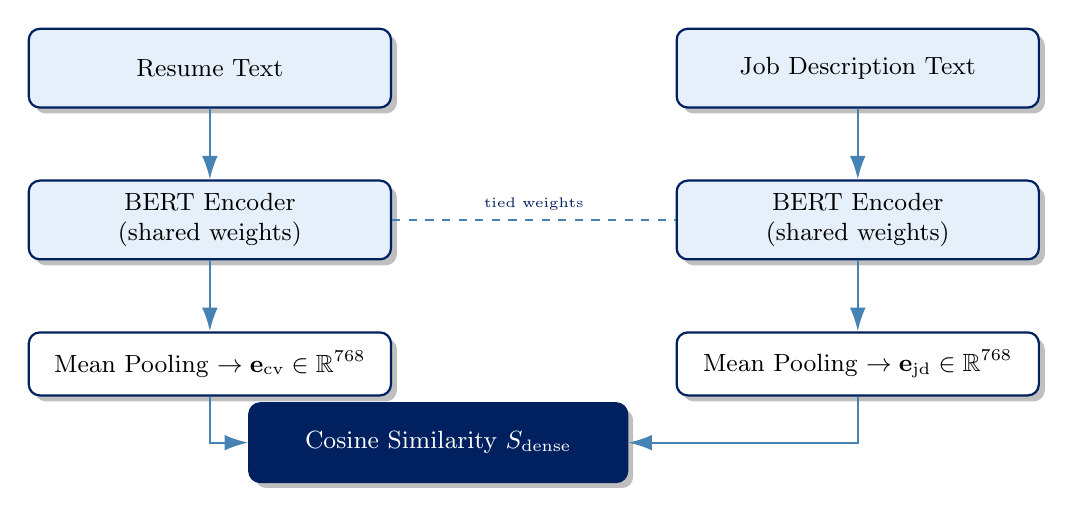
\begin{tikzpicture}[
        node distance=0.9cm and 1.4cm,
        box/.style={rectangle, draw=navyblue, fill=softblue, thick, rounded corners=4pt,
                    minimum width=4.6cm, minimum height=1.0cm, align=center, font=\small, drop shadow},
        poolbox/.style={rectangle, draw=navyblue, fill=white, thick, rounded corners=4pt,
                        minimum width=4.6cm, minimum height=0.8cm, align=center, font=\small, drop shadow},
        simbox/.style={rectangle, draw=navyblue, fill=navyblue, text=white, thick, rounded corners=4pt,
                       minimum width=4.8cm, minimum height=1.0cm, align=center, font=\small, drop shadow},
        arrow/.style={draw, -{Latex[length=3mm, width=2mm]}, thick, borderblue}
    ]
        \node [box] (cv) {Resume Text};
        \node [box, right=3.6cm of cv] (jd) {Job Description Text};
        \node [box, below=of cv]   (bert1) {BERT Encoder\\(shared weights)};
        \node [box, below=of jd]   (bert2) {BERT Encoder\\(shared weights)};
        \node [poolbox, below=of bert1] (pool1) {Mean Pooling $\to \mathbf{e}_{\text{cv}} \in \mathbb{R}^{768}$};
        \node [poolbox, below=of bert2] (pool2) {Mean Pooling $\to \mathbf{e}_{\text{jd}} \in \mathbb{R}^{768}$};
        \node [simbox, below=1.8cm of bert1, xshift=2.9cm] (sim) {Cosine Similarity $S_{\text{dense}}$};
        \path [arrow] (cv)    -- (bert1);
        \path [arrow] (jd)    -- (bert2);
        \path [arrow] (bert1) -- (pool1);
        \path [arrow] (bert2) -- (pool2);
        \path [arrow] (pool1) |- (sim);
        \path [arrow] (pool2) |- (sim);
        \path [draw, dashed, borderblue] (bert1) -- node[above, font=\tiny, text=navyblue]{tied weights} (bert2);
    \end{tikzpicture}%
    }
    \caption{The SBERT bi-encoder architecture: twin, weight-tied BERT towers independently embed each text, mean-pooling collapses token embeddings to a single 768-dimensional vector, and similarity is computed post-hoc via cosine distance.}
    \label{fig:sbert_biencoder}
\end{figure}

Two independent encoders process the resume and job description separately, requiring only a single forward pass each. I perform the ultimate comparison in $O(d)$ via cosine similarity afterwards, gracefully reducing the retrieval cost from quadratic to linear across the corpus.

\begin{remarkbox}{Why Not Use Raw BERT Token Averages?}
Reimers and Gurevych conclusively demonstrated that averaging raw BERT token outputs performs measurably \emph{worse} than rudimentary GloVe sentence averages on semantic benchmarks. BERT was originally trained for masked-language modeling and next-sentence prediction---tasks that do not naturally necessitate a geometrically coherent sentence-level embedding space. SBERT's Siamese fine-tuning (against classification or regression objectives on sentence-pair similarity data) is the precise mechanism that forces cosine angles to map directly to human-perceived semantic proximity. Without it, the geometric intuition underpinning $S_{\text{dense}}$ would be entirely invalid.
\end{remarkbox}

\subsection{The Hybrid OLS Blend: A Constrained Linear Ensemble}

To build a model that captures both deep semantic meaning and exact critical acronyms, I formulated the hybrid score $S_{\text{hybrid}} = w_0 + w_1 S_{\text{tfidf}} + w_2 S_{\text{dense}}$. I optimized this ensemble on the training split via Ordinary Least Squares (OLS): $\hat{\mathbf{w}} = (\mathbf{X}^\top\mathbf{X})^{-1}\mathbf{X}^\top\mathbf{y}$, where $\mathbf{X} = [\mathbf{1},\, S_{\text{tfidf}},\, S_{\text{dense}}]$. If the fitted $|w_2|$ heavily dominates $|w_1|$, the mathematics independently validate my core thesis that dense semantics are a substantially stronger predictor of candidate relevance than sparse lexical overlap.

\section{Ranking Mathematics: Pointwise, Pairwise, and Listwise Paradigms}
\label{sec:ranking_math}

\subsection{Pointwise Optimization: Why Regression Fails Candidate Sorting}

Phase 1 of my modeling pipeline evaluates standard Pointwise models (such as Ridge Regression and HistGradientBoosting) that seek to minimize Mean Squared Error (MSE):

\begin{equation}
\mathcal{L}_{\text{MSE}} = \frac{1}{N}\sum_{i=1}^{N}(y_i - \hat{y}_i)^2
\label{eq:mse}
\end{equation}

MSE treats each prediction in a vacuum, with no gradient term coupling $\hat{y}_i$ and $\hat{y}_j$ for candidates $i, j$ located within the same query group. Consider a scenario with Candidate A (true human score 0.71) and Candidate B (true human score 0.69). If the model predicts $\hat{y}_A = 0.65$ and $\hat{y}_B = 0.68$, the squared errors $(0.06)^2 + (0.01)^2$ are incredibly small, creating the illusion of high accuracy. Yet, the model has completely inverted the recruiter's intended ranking ($\hat{y}_B > \hat{y}_A$). Pointwise optimizers are fundamentally blind to list inversion, necessitating a shift to list-aware paradigms.

\subsection{Pairwise Optimization: The RankNet Probabilistic Model}
\label{subsec:ranknet}

RankNet (which forms the core logic inside \texttt{XGBRanker}) corrects this blindness by reframing ranking as pairwise classification. The probability that document $i$ is more relevant than document $j$ is mathematically modeled as a logistic sigmoid:

\begin{equation}
P_{ij} \equiv P(i \succ j) = \frac{1}{1 + e^{-\sigma(s_i - s_j)}}
\label{eq:ranknet_prob}
\end{equation}

\vspace{0.5em}

With ground-truth hierarchical labels $\bar{P}_{ij} = 1$ whenever $i$ is strictly more relevant, the network minimizes binary cross-entropy over all paired preferences:

\begin{equation}
C_{ij} = -\bar{P}_{ij}\log P_{ij} - (1-\bar{P}_{ij})\log(1-P_{ij})
\label{eq:ranknet_ce}
\end{equation}

\vspace{0.5em}

Substituting $\bar{P}_{ij}=1$ into Equation~\eqref{eq:ranknet_ce} simplifies the loss beautifully:

\begin{align}
C_{ij} = -\log P_{ij} = \log\!\left(1+e^{-\sigma(s_i-s_j)}\right)
\label{eq:ranknet_derivation}
\end{align}

\vspace{0.5em}

Summing this logarithmic loss over all relevant pairs in a localized query group $q$ recovers the exact pairwise loss optimized by \texttt{XGBRanker}:

\begin{equation}
\mathcal{L}_{\text{Pairwise}} = \sum_{i,j \in q} \log_2\!\left(1 + e^{-\sigma(s_i - s_j)}\right)
\label{eq:pairwise_loss}
\end{equation}

\subsection{Listwise Optimization: LambdaMART and NDCG Gradients}
\label{subsec:lambdamart}

While Pairwise optimization solves pointwise blindness, it carries its own structural flaw: it treats a ranking swap at position 99 identically to a swap at position 1. In real-world Human Resources, this is unacceptable; a recruiter will only ever read the top 10 resumes. LambdaMART (which drives \texttt{LGBMRanker}) resolves this by overriding the neural gradient directly:

\begin{equation}
\lambda_{ij} = \frac{\partial C_{ij}}{\partial s_i} = \frac{-\sigma}{1+e^{\sigma(s_i-s_j)}} \cdot \big|\Delta Z_{ij}\big|
\label{eq:lambda_gradient}
\end{equation}

\vspace{0.5em}

Here $|\Delta Z_{ij}|$ represents the absolute shift in a top-heavy Information Retrieval metric, specifically $\text{NDCG}@K$, if we were to swap candidates $i$ and $j$:

\begin{equation}
\text{NDCG}@K = \frac{\text{DCG}@K}{\text{IDCG}@K}, \quad \text{DCG}@K = \sum_{i=1}^{K}\frac{2^{\text{rel}_i}-1}{\log_2(i+1)}
\label{eq:ndcg}
\end{equation}

\vspace{0.5em}

Because the logarithmic denominator, $\log_2(i+1)$, acts as a severe decay penalty, $|\Delta Z_{ij}|$ is automatically massive for top-rank swaps and near zero for tail swaps. My model explicitly concentrates its optimization bandwidth exactly where it matters most: the elite shortlist.

\begin{insightbox}
The $|\Delta\text{NDCG}_{ij}|$ multiplier in Equation~\eqref{eq:lambda_gradient} is the precise mathematical mechanism driving \texttt{LGBMRanker}'s superiority over \texttt{XGBRanker} in the empirical evaluations (Section~\ref{ch:results}). Both utilize the same underlying pairwise probability model, but only LambdaMART dynamically re-weights its gradient by rank-position sensitivity, forcing the algorithm to obsess over the Top-10 candidates.
\end{insightbox}

\section{Information Retrieval Evaluation: Spearman's Rank Correlation}
\label{sec:spearman_theory}

\begin{definitionbox}{Spearman's Rank Correlation ($\rho$)}
Given a set of $n$ paired observations with rank discrepancies defined as $d_i = R_{X_i} - R_{Y_i}$:
\begin{equation}
\rho = 1 - \frac{6\sum_{i=1}^{n} d_i^2}{n(n^2-1)}
\label{eq:spearman}
\end{equation}
This is statistically equivalent to computing the standard Pearson correlation directly on the rank ordinals, $\rho = \text{Pearson}\big(\text{rank}(X), \text{rank}(Y)\big)$.
\end{definitionbox}

\vspace{0.5em}

\paragraph{Derivation.} Since $R_X$ and $R_Y$ are both permutations of the integer sequence $\{1,\ldots,n\}$, they share a predictable mean $\bar{R} = \frac{n+1}{2}$ and a strict sum of squared deviations $\frac{n(n^2-1)}{12}$. By geometrically expanding the squared rank discrepancy $\sum_i d_i^2$:

\begin{align}
\sum_i d_i^2 &= 2\cdot\frac{n(n^2-1)}{12} - 2\sum_i (R_{X_i}-\bar R)(R_{Y_i}-\bar R)
\label{eq:spearman_exp}
\end{align}

\vspace{0.5em}

I isolate the covariance-style cross term. Substituting this directly into the standard Pearson correlation formula allows the terms to collapse seamlessly:

\begin{equation}
\rho = \frac{\frac{n(n^2-1)}{12} - \frac{1}{2}\sum_i d_i^2}{\frac{n(n^2-1)}{12}} = 1 - \frac{6\sum_i d_i^2}{n(n^2-1)}
\label{eq:spearman_proof}
\end{equation}

Spearman's $\rho$ penalizes rank discrepancies uniformly across all list positions, whereas $\text{NDCG}@K$ overwhelmingly down-weights errors below rank $K$ and ignores everything beyond it. Reporting both metrics simultaneously allows me to distinguish a ``globally stable hierarchical ordering'' from a ``highly accurate top-10 shortlist''---which represent distinct, practically important business claims.

\section{Feature Engineering: The Experience Gap as a Bayesian Inference Problem}
\label{sec:deltaE_theory}

The semantic matching framework of Sections~\ref{sec:vsm}--\ref{sec:spearman_theory} accurately captures textual skill overlap, but ignores a second orthogonal signal: temporal fit. A candidate can be a perfect semantic match for a role but still be wholly unsuitable if they lack the minimum tenure required. I define this \emph{experience gap} as:

\begin{equation}
\Delta E = \text{Exp}_{\text{cand}} - \text{Exp}_{\text{req}}
\label{eq:delta_e_def}
\end{equation}

\vspace{0.5em}

Converting this raw numerical gap into a score adjustment requires a penalty function whose \emph{shape} mathematically encodes assumptions about recruiter risk perception. I formulate and rigorously compare three competing shapes.

\subsection{The Cold-Start Problem: Why This Is a Bayesian Inference Task}
\label{sec:cold_start}
\label{subsec:bayes_motivation}

In a mature, data-rich HR system, the natural statistical question is: ``What is the empirical probability that a candidate with $\Delta E = -3$ years succeeds in this role?'' I could answer this directly if I had access to a massive historical table of hire decisions and post-hire performance outcomes---a true empirical Bayesian likelihood table, $P(\text{success} \mid \Delta E\text{ bucket})$, calculated from real data.

My dataset---and virtually every open-source academic recruitment corpus---does not carry this longitudinal information. The Neuralframe AI resume dataset contains resume text and job descriptions; it does not contain historical outcome labels (Was this candidate hired? Did they pass probation?). Building an empirical Bayesian table requires tracking actual hiring decisions across thousands of roles over several years, data that only exists at the enterprise institutional scale.

This represents the classic \textbf{cold-start problem} in applied Bayesian statistics. The standard response is not to abandon probabilistic inference entirely, but to:

\begin{enumerate}[noitemsep]
    \item Replace the missing empirical likelihood with a \textbf{parametric approximation} whose shape mathematically encodes the qualitative behavior I believe the true relationship possesses.
    \item Use whatever informative signal \textbf{is} available (the NLP semantic extraction) as the prior.
    \item Design the architecture to be \textbf{upgradable}: once enough longitudinal hiring outcome data accumulates, the parametric approximation can be instantly swapped for a fitted empirical function without breaking anything downstream.
\end{enumerate}

\vspace{0.5em}

This is precisely why I chose a Sigmoid function as the likelihood approximation (Section~\ref{subsec:sigmoid_bayes}): it is the natural parametric form for ``a probability that changes monotonically with a continuous predictor'', and it belongs to the same functional family underlying logistic regression---a principled statistical choice, not merely an aesthetic one.

\subsection{Method A: The Linear Baseline}
\label{subsec:method_a}

\begin{definitionbox}{Linear Penalty}
\begin{equation}
\text{Penalty}_{\text{linear}}(\Delta E) =
\begin{cases}
k \cdot \Delta E, & \Delta E < 0 \\
0, & \Delta E \ge 0
\end{cases}
\label{eq:linear_penalty}
\end{equation}
with $k = 0.05$ and providing no mathematical credit for surplus experience.
\end{definitionbox}

This serves as the industry baseline---it represents the underlying logic that most legacy, commodity ATS platforms effectively execute when they subtract points for experience shortfalls. Its primary virtue is transparent simplicity: every missing year of experience costs exactly $k$ points, with no hidden nonlinearities. I established this model strictly as a performance floor; my advanced formulations must logically and empirically outperform this trivial rule to justify their added computational complexity.

\subsection{Method B: The Piecewise Quadratic Penalty (Deployed)}
\label{subsec:method_b}

\begin{definitionbox}{Piecewise Quadratic-Linear Penalty}
\begin{equation}
\text{Penalty}_{\text{quad}}(\Delta E) =
\begin{cases}
-\alpha \cdot (\Delta E)^2, & \Delta E < 0 \quad (\text{under-qualified}) \\
+\beta \cdot \Delta E, & \Delta E \ge 0 \quad (\text{requirement met})
\end{cases}
\label{eq:quadratic_penalty}
\end{equation}
Through iterative calibration on the training split, I empirically fixed these hyperparameters to $\alpha = 0.04$ and $\beta = 0.01$.
\end{definitionbox}

The quadratic term successfully encodes a genuine asymmetry in recruiter risk perception: a candidate missing four years of experience is not perceived as merely ``twice as bad'' as one missing two years---the perceived risk accelerates disproportionately. The small linear surplus reward ($\beta = 0.01$) rewards tenure without allowing over-qualified candidates to uniformly overshadow substantially better technical matches.

\paragraph{The Saturation Threshold.} However, the quadratic formulation introduces a mathematically verifiable failure mode in the deficit tail. Given a baseline semantic $\texttt{Match\_Score} = m$, the adjusted score first crashes into the zero floor at:

\begin{equation}
m - \alpha(\Delta E^*)^2 = 0 \implies \Delta E^* = -\sqrt{\frac{m}{\alpha}}
\label{eq:quad_threshold}
\end{equation}

\vspace{0.5em}

For $m = 0.75$ and $\alpha = 0.04$: $\Delta E^* = -\sqrt{18.75} \approx -4.33$ years. Beyond this point, every candidate clips to an identical adjusted score of $0.0$, regardless of how much further below the threshold they fall. For a split-based learner like \texttt{LGBMRanker}, a feature that remains constant over a subrange carries \textbf{zero} information gradient for differentiating candidates within that dead zone.

\subsection{Method C: The Sigmoid-Bayesian Posterior (Proposed)}
\label{subsec:sigmoid_bayes}

To overcome the saturation failure, I constructed a probabilistic model using the existing \texttt{Match\_Score} as a semantic prior and the Sigmoid function as the parametric likelihood approximation.

\begin{definitionbox}{Prior: Semantic Competence Belief}
\begin{equation}
P(C) = \texttt{Match\_Score} \in (0,1)
\label{eq:prior}
\end{equation}
The prior probability that a candidate is competent is taken directly from the SBERT semantic similarity score. This ensures experience is never evaluated in a vacuum; the baseline belief is fundamentally anchored in the candidate's actual extracted technical vocabulary.
\end{definitionbox}

\begin{definitionbox}{Sigmoid Likelihood}
\begin{equation}
L(\Delta E) = \frac{1}{1 + e^{-k_s(\Delta E - \delta)}}
\label{eq:sigmoid_likelihood}
\end{equation}
This approximates $P(\text{observing this gap} \mid \text{candidate is competent})$ via a logistic decay curve. $k_s > 0$ controls the steepness of decay per year of shortfall; $\delta$ sets the inflection point (where ``meeting the requirement'' transitions from neutral to positive evidence). Mirroring the calibration procedure used for Method B, I fixed $k_s = 0.35$ and $\delta = 0$ on the training split, placing the neutral-evidence point exactly at $\Delta E = 0$.
\end{definitionbox}

\begin{definitionbox}{Posterior via Bayes' Rule}
\begin{equation}
P(C \mid \Delta E) = \frac{L(\Delta E)\, P(C)}{L(\Delta E)\, P(C) + \big(1 - L(\Delta E)\big)\big(1 - P(C)\big)}
\label{eq:bayes_posterior}
\end{equation}
This relies on the standard Naive-Bayes assumption that the complementary hypothesis is evidenced by $1 - L(\Delta E)$.
\end{definitionbox}

\paragraph{The Log-Odds Identity.} To truly understand why this Bayesian fusion works, we must look at its log-odds transformation. Writing $\operatorname{logit}(p) = \ln\big(\tfrac{p}{1-p}\big)$, algebraic rearrangement gives:

\begin{align}
\operatorname{logit}\big(P(C \mid \Delta E)\big)
&= \ln\!\left(\frac{L(\Delta E)}{1-L(\Delta E)}\right) + \ln\!\left(\frac{P(C)}{1-P(C)}\right) \notag \\
&= \operatorname{logit}\big(L(\Delta E)\big) + \operatorname{logit}\big(P(C)\big)
\label{eq:log_odds_identity}
\end{align}

\vspace{0.5em}

The posterior log-odds is exactly equal to the \emph{sum} of the prior log-odds and the likelihood log-odds. This additive evidence-pooling identity is the mathematical engine powering logistic scorecards and Naive-Bayes classifiers. It allows me to seamlessly fuse two completely independent signals (NLP semantic fit and temporal experience fit) onto a shared, probabilistically sound log-odds scale, rather than arbitrarily subtracting a penalty from a similarity score.

\begin{figure}[htbp]
    \centering
    \resizebox{0.95\linewidth}{!}{%
    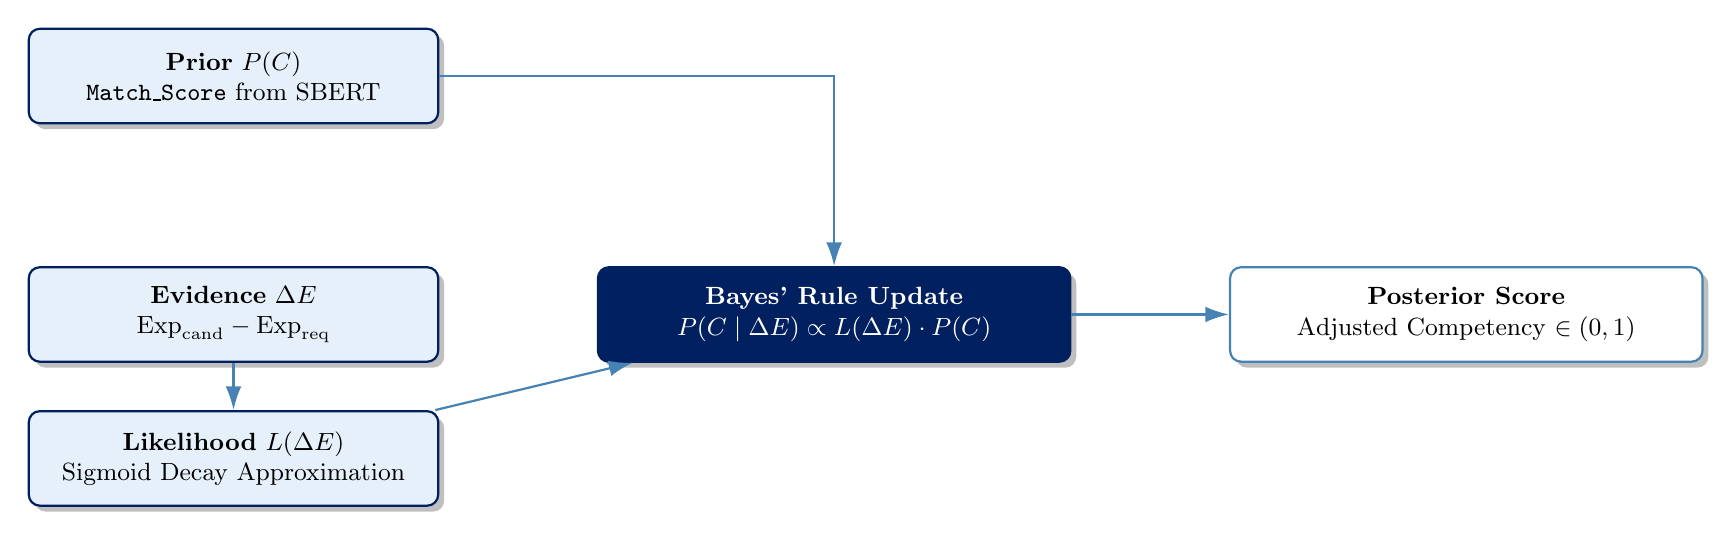
\begin{tikzpicture}[
        node distance=1.0cm and 1.6cm,
        box/.style={rectangle, draw=navyblue, fill=softblue, thick, rounded corners=4pt,
                    minimum width=5.2cm, minimum height=1.2cm, align=center, font=\small, drop shadow},
        bayesbox/.style={rectangle, draw=navyblue, fill=navyblue, text=white, thick, rounded corners=4pt,
                         minimum width=6.0cm, minimum height=1.2cm, align=center, font=\small, drop shadow},
        outbox/.style={rectangle, draw=borderblue, fill=white, thick, rounded corners=4pt,
                       minimum width=6.0cm, minimum height=1.2cm, align=center, font=\small, drop shadow},
        arrow/.style={draw, -{Latex[length=3mm, width=2mm]}, thick, borderblue}
    ]
        \node [box] (prior)      {\textbf{Prior} $P(C)$\\\texttt{Match\_Score} from SBERT};
        \node [box, below=1.8cm of prior] (evidence)   {\textbf{Evidence} $\Delta E$\\$\text{Exp}_{\text{cand}} - \text{Exp}_{\text{req}}$};
        \node [box, below=0.6cm of evidence] (likelihood) {\textbf{Likelihood} $L(\Delta E)$\\Sigmoid Decay Approximation};
        \node [bayesbox, right=2.0cm of evidence] (bayes) {\textbf{Bayes' Rule Update}\\$P(C \mid \Delta E) \propto L(\Delta E) \cdot P(C)$};
        \node [outbox, right=2.0cm of bayes]      (posterior) {\textbf{Posterior Score}\\Adjusted Competency $\in (0,1)$};
        \path [arrow] (prior)      -| (bayes);
        \path [arrow] (evidence)   -- (likelihood);
        \path [arrow] (likelihood) -- (bayes);
        \path [arrow] (bayes)      -- (posterior);
    \end{tikzpicture}%
    }
    \caption{Bayesian evidence-combination DAG for the Sigmoid-Bayesian $\Delta E$ model. The semantic prior and the experience-derived likelihood are fused multiplicatively via Bayes' rule rather than added as independent penalty terms, allowing the same gap to produce different adjustments depending on the underlying prior strength.}
    \label{fig:bayesian_logic}
\end{figure}

\subsection{Asymptotic Tail Analysis}
\label{sec:tail_analysis}

\paragraph{Method B reaches a hard floor at finite $\Delta E$.} As derived in Equation~\eqref{eq:quad_threshold}, every candidate with $\Delta E < \Delta E^* \approx -4.33$ years clips to an identical adjusted score of $0.0$. Two candidates at $\Delta E = -4.5$ and $\Delta E = -9$ become computationally indistinguishable; the feature carries zero discriminative variance in that region.

\paragraph{Method C decays asymptotically but never terminates.} As $\Delta E \to -\infty$, I expand the sigmoid approximation asymptotically:

\begin{equation}
L(\Delta E) \sim e^{k_s(\Delta E - \delta)} \quad \text{as } \Delta E \to -\infty
\label{eq:sigmoid_asymptotic}
\end{equation}

\vspace{0.5em}

By substituting this into Equation~\eqref{eq:bayes_posterior}:

\begin{equation}
P(C \mid \Delta E) \sim \frac{P(C)}{1-P(C)}\, e^{k_s(\Delta E - \delta)} \quad \text{as } \Delta E \to -\infty
\label{eq:posterior_asymptotic}
\end{equation}

\vspace{0.5em}

The posterior decays \emph{exponentially} toward---but never hits---zero. Candidates at $\Delta E = -4.5$ and $\Delta E = -9$ differ by a factor of $e^{4.5 k_s}$ in their posteriors, preserving the ranking hierarchy. Method C maintains ranking-relevant information across the \emph{entire} real line, whereas Method B provably obliterates it beyond a threshold well within the observed applicant pool.

\begin{insightbox}
The key statistical advantage of the Sigmoid-Bayesian formulation is not just that it avoids a flat gradient region, but that the \emph{same} experience gap produces a \emph{different} posterior adjustment depending on the prior \texttt{Match\_Score}. A highly qualified candidate ($\texttt{Match\_Score} = 0.91$) with $\Delta E = -4.5$ years retains a posterior of $0.677$---the strong semantic prior rescues part of the confidence. A weak semantic match ($\texttt{Match\_Score} = 0.65$) with the exact same gap would fall substantially lower. Methods A and B, being purely additive, completely fail to express this interaction.
\end{insightbox}

\subsection{Mathematical and Behavioral Comparison}
\label{sec:deltaE_comparison}

Table~\ref{tab:method_comparison_math} summarizes the three formulations across the dimensions most relevant to their performance as \texttt{LGBMRanker} input features.

\begin{table}[H]
    \centering
    \caption{Mathematical and behavioral comparison of the three $\Delta E$ penalty formulations.}
    \label{tab:method_comparison_math}
    \small
    \begin{tabular}{>{\raggedright\arraybackslash}p{2.5cm}>{\raggedright\arraybackslash}p{3.4cm}>{\raggedright\arraybackslash}p{3.4cm}>{\raggedright\arraybackslash}p{3.8cm}}
        \toprule
        & \textbf{Linear (A)} & \textbf{Quadratic (B)} & \textbf{Sigmoid-Bayesian (C)} \\
        \midrule
        Output range & Unbounded (clipped) & Unbounded (clipped) & Naturally bounded $(0,1)$ \\
        Deficit tail & Constant marginal penalty & Accelerating, clips to $0$ at $\Delta E^*$ & Exponential asymptotic decay \\
        Surplus tail & No reward & Small linear reward & Diminishing-returns reward \\
        Free params & $1$ ($k$) & $2$ ($\alpha, \beta$) & $2$ ($k_s, \delta$), probabilistically interpretable \\
        Interaction with prior & None (additive) & None (additive) & Multiplicative via Bayes' rule \\
        Interpretability & Very high & High & Moderate (needs translation) \\
        \bottomrule
    \end{tabular}
\end{table}

To synthesize the theoretical groundwork laid out in this section, Table~\ref{tab:theory_summary} explicitly maps every mathematical construct I derived---from text vectorization to listwise ranking and Bayesian inference---to its specific empirical application within my deployed screening architecture. By grounding the pipeline in these proven statistical principles rather than relying on heuristic string-matching rules, the system moves beyond arbitrary ATS filtering. The mathematical models derived here ensure that the final algorithmic decisions---whether embedding a semantic concept or dynamically penalizing a tenure shortfall---are verifiable, globally stable, and structurally designed to optimize for an elite candidate shortlist.

\begin{table}[H]
\centering
\caption{Theoretical foundations and their empirical applications in the CV screening architecture.}
\label{tab:theory_summary}
\small
\begin{tabular}{@{}>{\raggedright\arraybackslash}p{4.2cm}>{\raggedright\arraybackslash}p{3.4cm}>{\raggedright\arraybackslash}p{5.0cm}@{}}
\toprule
\textbf{Theoretical Concept} & \textbf{Equation Form} & \textbf{Applied Pipeline Stage} \\
\midrule
TF-IDF Keyword Weighting & \eqref{eq:tfidf} & Lexical extraction ($S_{\text{tfidf}}$) \\
Cosine Similarity & \eqref{eq:cosine_sim} & Vector matching ($S_{\text{tfidf}},S_{\text{dense}}$) \\
Self-Attention Mechanism & \eqref{eq:attention} & \texttt{nomic-embed-text-v1.5} encoder \\
Pointwise MSE Constraints & \eqref{eq:mse} & Regression Phase 1 baselines \\
RankNet Pairwise Loss & \eqref{eq:pairwise_loss} & \texttt{XGBRanker} optimization \\
LambdaMART Gradient & \eqref{eq:lambda_gradient} & \texttt{LGBMRanker} optimization \\
Spearman's $\rho$ & \eqref{eq:spearman} & LTR global stability evaluation \\
Linear Penalty & \eqref{eq:linear_penalty} & $\Delta E$ baseline (Method A) \\
Quadratic Penalty & \eqref{eq:quadratic_penalty} & $\Delta E$ deployed (Method B) \\
Sigmoid-Bayesian Posterior & \eqref{eq:bayes_posterior} & $\Delta E$ proposed (Method C) \\
Log-Odds Identity & \eqref{eq:log_odds_identity} & Bayesian combination proof \\
\bottomrule
\end{tabular}
\end{table}

By grounding the pipeline in these proven statistical principles rather than relying on heuristic string-matching rules, the system moves beyond arbitrary ATS filtering. The mathematical models derived here ensure that the final algorithmic decisions---whether embedding a semantic concept or dynamically penalizing a tenure shortfall---are verifiable, globally stable, and structurally designed to optimize for an elite candidate shortlist.
\chapter{Aims \& Objectives}
\label{sec:objectives}

To push past the limitations of traditional keyword extraction, I anchored this initiative around five primary technical and statistical objectives:

\begin{enumerate}[topsep=4pt, itemsep=4pt]
    \item \textbf{Develop a Robust NLP Pipeline:} Transition from brittle, sparse lexical arrays (TF-IDF) to \textbf{dense semantic tensors}. By applying morphological lemmatization and domain-specific blocklists, I isolate genuine technical signals before projecting candidate profiles into a geometric space using \textbf{SBERT bi-encoders}.
    
    \item \textbf{Enforce Data Leakage Prevention:} Eliminate the risk of vocabulary memorization by constructing a strict \textbf{\texttt{GroupShuffleSplit}} architecture. Partitioning the training and test matrices by discrete job roles mathematically guarantees the pipeline is evaluated strictly on its true \textbf{zero-shot generalization} capabilities.
    
    \item \textbf{Benchmark Baseline Estimators:} Expose the structural blindness of pointwise regression (MSE) and threshold-based binary classification (BCE), empirically proving that \textbf{predicting absolute relevance scores fails} to capture the inherently comparative, ordinal nature of human recruitment.
    
    \item \textbf{Deploy Listwise LTR Frameworks:} Shift the optimization objective to top-heavy Information Retrieval metrics (\textbf{NDCG@10}) by evaluating gradient-boosted ranking estimators. I specifically contrast pairwise probability networks (\textbf{\texttt{XGBRanker}}) against listwise LambdaMART gradient scaling (\textbf{\texttt{LGBMRanker}}).
    
    \item \textbf{Mathematically Model the Experience Gap ($\Delta E$):} Formalize recruiter intuition regarding tenure mismatches by replacing ad-hoc HR rules with \textbf{probabilistically sound functions}. I construct and evaluate a piecewise quadratic threshold against a novel \textbf{Sigmoid-Bayesian posterior} to handle temporal fit under data-scarce (cold-start) conditions.
\end{enumerate}


\subsection{Engineering Relevance and Statistical Integrity}
\label{subsec:engineering_relevance}

It is important to clarify the true scope of this work. I did not approach this project as a mere software engineering exercise---simply wiring APIs together to build a dashboard. Instead, my primary focus was on ensuring \textbf{empirical validity, algorithmic fairness, and statistical integrity}.

When applying machine learning to human resources, the risk of \textbf{data leakage and training--serving skew} is exceptionally high. If I had trained the algorithm on a random split of resumes, it would likely have just memorized the specific vocabulary of the job postings in the training set. Consequently, if deployed in production against a brand-new job description, its predictive performance would completely collapse. To eliminate this vulnerability, I implemented strict \textbf{\texttt{GroupShuffleSplit} validation architectures}, which actively forced my models to evaluate \textbf{completely unseen job groups}.

Furthermore, standard pointwise regression models are statistically ill-equipped for recruitment. Predicting that a candidate is an ``85\% match'' is meaningless in a vacuum. Recruitment is inherently a \textbf{sorting problem}---the true goal is to identify the \textbf{best relative fit} within a specific applicant pool. By benchmarking continuous regression against binary classification, and ultimately deploying specialized \textbf{Learning-to-Rank (LTR) gradient estimators}, I was able to rigorously isolate the optimal mathematical framework for \textbf{human-centric candidate ranking}.
\chapter{Methodology}
\label{ch:methodology}

Before deploying the complex semantic embedding models and Learning-to-Rank estimators, it was imperative that I construct a highly sanitized, empirically stable data foundation alongside an experimental design that honestly simulates a real-world Human Resources deployment. In this section, I detail the ingestion of the raw corpus, the rigorous linguistic filtering I executed via \texttt{spaCy}, the Exploratory Data Analysis (EDA) that drove my feature engineering decisions, and the strict partitioning logic I used to prevent target leakage. Finally, I outline my \textbf{Tri-Framing modeling framework} and the mathematical metrics I used to benchmark algorithmic success.

\section{Data Source, Ingestion, and Schema}
\label{sec:data_source}

I derived the foundational data for this study from an open-source recruitment corpus compiled by Neuralframe AI and published on Kaggle. The raw ingestion file (\texttt{resume\_data.csv}) constitutes a 17 MB dataset comprising $9{,}544$ candidate records. Distributed under the Creative Commons CC BY-NC 4.0 license, the corpus provides highly granular professional profiles, including unstructured text fields for career objectives, technical skills, educational background, and employment histories, mapped against specific job postings.

To process this for my automated pipeline, I transformed the raw corpus into an engineered schema, yielding the primary working file, \texttt{ml\_ready\_dataset.csv}. Table~\ref{tab:dataset_schema} outlines the core features I engineered during ingestion that pass into the modeling phases.

\begin{table}[htbp]
\centering
\caption{Core schema architecture for the engineered \texttt{ml\_ready\_dataset.csv}.}
\label{tab:dataset_schema}
\small
\renewcommand{\arraystretch}{1.5} % Increased row spacing for better readability
\begin{tabular}{@{}>{\raggedright\arraybackslash}p{3.0cm}>{\raggedright\arraybackslash}p{2.5cm}>{\raggedright\arraybackslash}p{8.5cm}@{}}
\toprule
\textbf{Feature Name} & \textbf{Data Type} & \textbf{Description / Engineering Logic} \\
\midrule
\texttt{Resume\_Text} & String (Text) & The fully concatenated, structurally sanitized corpus of the candidate's professional profile. \\
\texttt{Job\_Desc} & String (Text) & The sanitized requirements and qualifications of the target job posting. \\
\texttt{Job\_Title} & Categorical & The specific role classification (e.g., Software Engineer, HR Manager), spanning 28 distinct groups. \\
\texttt{Exp\_cand} & Float (Years) & Parsed aggregate years of professional experience possessed by the candidate. \\
\texttt{Exp\_req} & Float (Years) & Minimum years of experience demanded by the job posting. \\
\texttt{Delta\_E} & Float (Years) & The calculated experience mismatch ($\text{Exp}_{\text{cand}} - \text{Exp}_{\text{req}}$). \\
\texttt{Match\_Score} & Float [0, 1] & Ground-truth relevance score or historical baseline SBERT semantic similarity. \\
\bottomrule
\end{tabular}
\end{table}

\section{Linguistic Sanitization and Dimensionality Reduction}
\label{sec:text_cleaning}

Raw resumes and corporate job descriptions represent some of the most chaotic unstructured text in modern data science. They are heavily polluted with inconsistent structural formatting, non-standard unicode characters, HTML artifacts, and ubiquitous corporate buzzwords that actively obscure a candidate's genuine technical qualifications.

If I passed this raw text directly into the TF-IDF or SBERT vectorizers, the mathematical space would become severely distorted by \textbf{semantic noise}. To combat this, I architected a central text-cleaning pipeline inside \texttt{utils.py}, utilizing the \texttt{spaCy} natural language processing library to enforce strict morphological sanitization, as illustrated in Figure~\ref{fig:nlp_pipeline}.

\begin{figure}[htbp]
    \centering
    \resizebox{0.95\linewidth}{!}{%
    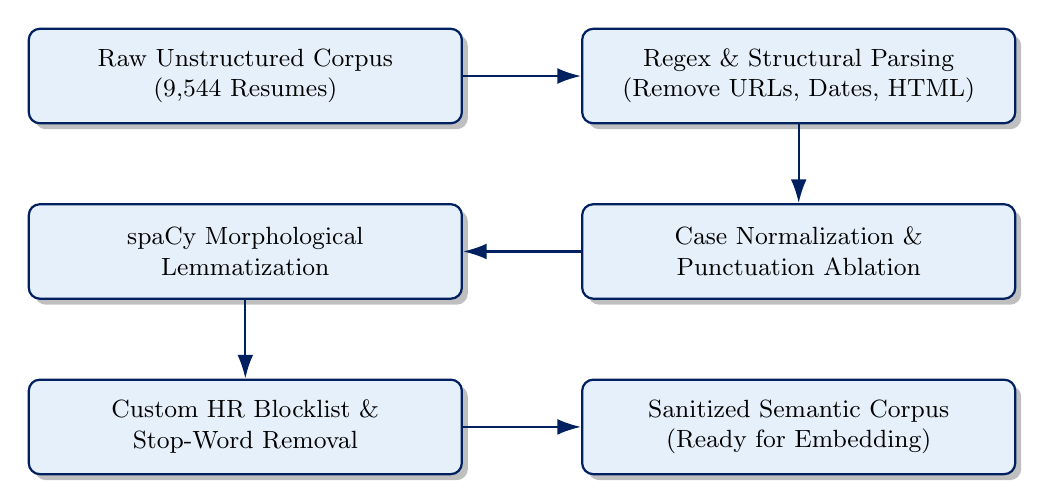
\begin{tikzpicture}[
        node distance=1.0cm and 1.5cm,
        box/.style={rectangle, draw=navyblue, fill=softblue, thick, rounded corners=4pt, minimum width=5.5cm, minimum height=1.2cm, align=center, font=\small, drop shadow},
        arrow/.style={draw, -{Latex[length=3mm, width=2mm]}, thick, navyblue}
    ]
        \node [box] (raw) {Raw Unstructured Corpus\\(9,544 Resumes)};
        \node [box, right=of raw] (regex) {Regex \& Structural Parsing\\(Remove URLs, Dates, HTML)};
        \node [box, below=of regex] (lower) {Case Normalization \&\\Punctuation Ablation};
        \node [box, left=of lower] (spacy) {spaCy Morphological\\Lemmatization};
        \node [box, below=of spacy] (stop) {Custom HR Blocklist \&\\Stop-Word Removal};
        \node [box, right=of stop] (clean) {Sanitized Semantic Corpus\\(Ready for Embedding)};

        \path [arrow] (raw) -- (regex);
        \path [arrow] (regex) -- (lower);
        \path [arrow] (lower) -- (spacy);
        \path [arrow] (spacy) -- (stop);
        \path [arrow] (stop) -- (clean);
    \end{tikzpicture}%
    }
    \caption{The sequential NLP sanitization pipeline designed to systematically reduce vocabulary dimensionality.}
    \label{fig:nlp_pipeline}
\end{figure}

My pipeline executes three primary transformations:
\begin{enumerate}
    \item \textbf{Structural Sanitization via Regular Expressions:} I programmatically stripped out metadata that holds zero predictive validity for technical competence, such as hyperlinks, physical addresses, and certificate dates.
    \item \textbf{Morphological Lemmatization:} Utilizing \texttt{spaCy}'s \texttt{en\_core\_web\_sm} model, I lowercased every document, stripped it of punctuation, and reduced it to its base lemmas.
    \item \textbf{Custom Stop-Word Ablation:} Beyond standard English stop-words, I curated a domain-specific blocklist of over 50 pervasive HR phrases (e.g., ``team player'', ``synergy''), whose Term Frequency approaches maximum density, rendering their Inverse Document Frequency zero.
\end{enumerate}

\section{Exploratory Data Analysis (EDA)}
\label{sec:eda}

\subsection{Bounding the Vector Space: Token Length Filtering}
Transformer-based models typically possess a strict maximum context window of 512 tokens. I defined empirical boundaries to manage this: I dropped records containing fewer than $20$ words as insufficient, and I truncated or dropped records exceeding $350$ words to prevent computational truncation artifacts.

\begin{figure}[htbp]
    \centering
    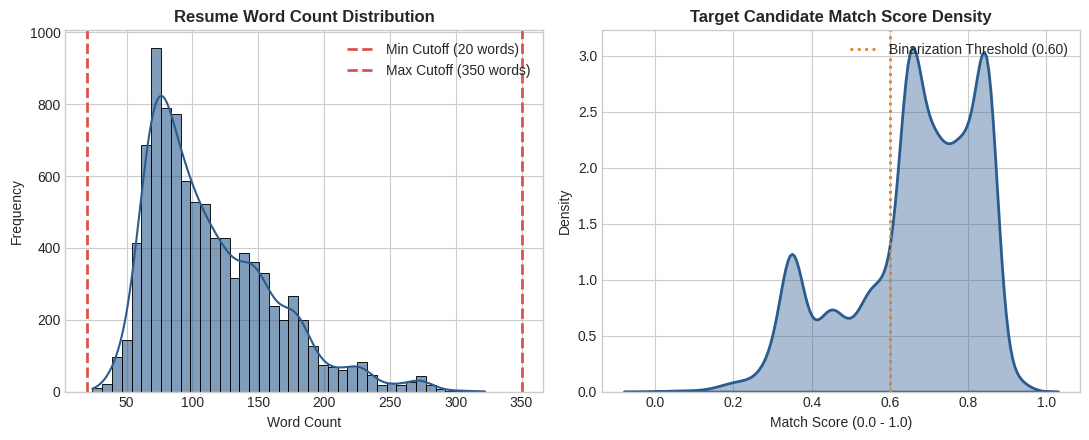
\includegraphics[width=0.95\linewidth]{density.png}
    \caption{Resume word-count filtering boundaries (left) and bimodal target-score density (right).}
    \label{fig:eda_density}
\end{figure}

As depicted in Figure~\ref{fig:eda_density}, the word-count distribution reveals a log-normal shape, clustering primarily between 75 and 150 words. My final sanitized dataset comprised $9{,}369$ high-quality records mapping to $28$ distinct job categories.

\subsection{Bimodal Density and Threshold Mechanics}
The right panel of Figure~\ref{fig:eda_density} plots the density of the target semantic match scores, revealing a bimodal distribution where a massive cluster of generic applicants scores between $0.20$ and $0.40$, and qualified shortlists cluster around $0.60$ to $0.85$.

\section{Corpus Vocabulary and Frequency Dynamics}
\label{subsec:vocab}

To confirm the sanitization pipeline (Section~\ref{sec:text_cleaning}) preserved the corpus's genuine technical signal rather than stripping it away, the surviving vocabulary was inspected directly, both qualitatively and quantitatively.

\begin{figure}[htbp]
    \centering
    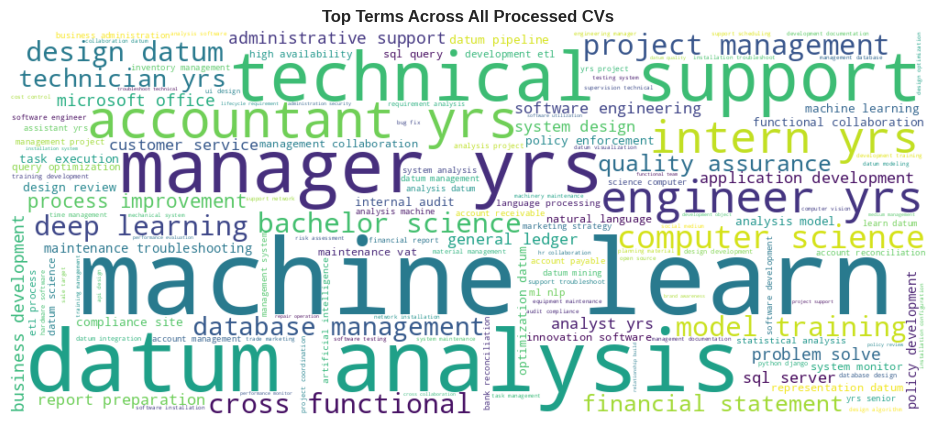
\includegraphics[width=0.85\linewidth]{word_cloud.png}
    \caption{Word cloud highlighting the prominent domain keywords extracted post-sanitization.}
    \label{fig:wordcloud}
\end{figure}

Figure~\ref{fig:wordcloud} gives a qualitative first read: font size scales with raw frequency, and the surviving vocabulary is dominated by concrete role and skill terms (\textit{manager}, \textit{engineer}, \textit{machine learn}, \textit{data analysis}) rather than the generic HR filler the blocklist was designed to remove. This is a useful sanity check, but a word cloud alone cannot support any quantitative claim, so the same vocabulary was re-examined as a ranked frequency count.

\begin{figure}[htbp]
    \centering
    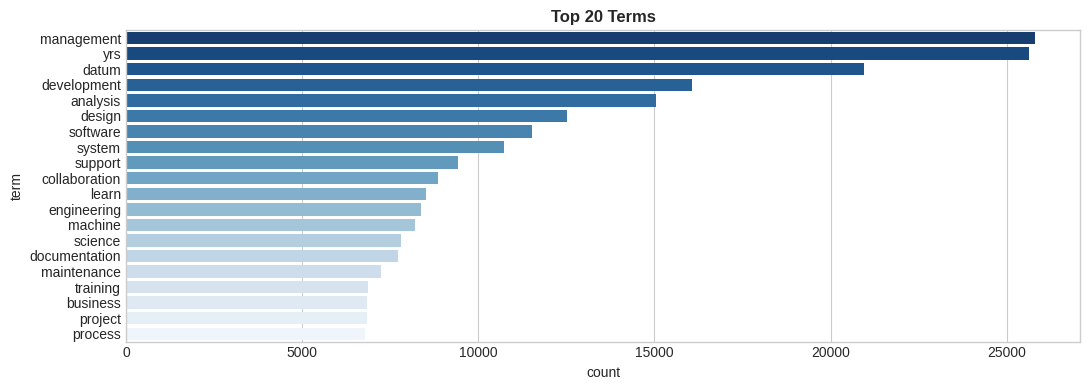
\includegraphics[width=0.95\linewidth]{word_bar.png}
    \caption{Absolute term frequency distribution for the top 20 computational and operational $n$-grams.}
    \label{fig:wordbar}
\end{figure}

Figure~\ref{fig:wordbar} makes that same picture numerically precise: \textit{management} and \textit{data} alone account for tens of thousands of occurrences each, with a long, gradually decaying tail down to more specialized terms like \textit{documentation} and \textit{process}. Together, Figures~\ref{fig:wordcloud} and~\ref{fig:wordbar} confirm that the dominant vectors remaining in the corpus are highly relevant terms like \textit{management}, \textit{data}, \textit{software}, and \textit{engineering} --- exactly the discriminative signal the TF-IDF and SBERT stages downstream depend on.

\section{Data Leakage Prevention via Group-Aware Splitting}
\label{sec:group_split}

When I initially approached the partitioning of the sanitized resume dataset, I identified a catastrophic risk: \textbf{target data leakage}. Standard machine learning pipelines universally default to randomized splitting architectures, such as \texttt{train\_test\_split}. In the context of candidate--job matching, employing a random split is empirically invalid.

Consider a scenario where 300 candidates apply for a specific ``Data Engineer'' vacancy. A random 80/20 split would allocate roughly 240 of these resumes to the training matrix and 60 to the hold-out test matrix. During training, the models would simply \textbf{memorize the highly specific, idiosyncratic vocabulary} associated with that exact ``Data Engineer'' job description, rather than learning the generalized geometric mapping between applicant skills and role requirements. When evaluated on the 60 test resumes, the model would produce artificially inflated accuracy scores. However, if deployed in a production ATS against a newly opened, previously unseen ``Financial Analyst'' role, the model's predictive capability would completely collapse.

To enforce a genuine \textbf{zero-shot generalization test}, I discarded random splitting in favor of a strict \textbf{\texttt{GroupShuffleSplit}}, using the \texttt{Job\_Title} target as the discrete grouping identifier. Letting $G_j$ represent the set of all candidate resumes applying for job $j$, I formalize this strict group-aware isolation as:
\begin{equation}
\left(\bigcup_{j \in \text{Train}} G_j\right) \cap \left(\bigcup_{k \in \text{Test}} G_k\right) = \varnothing
\label{eq:disjoint_split}
\end{equation}

By executing this architecture, I successfully partitioned $7{,}356$ rows (encompassing 22 distinct job postings) exclusively into the training set. I strictly populated the test set with $2{,}013$ rows mapped against 6 completely unseen job roles. Furthermore, I fitted all sparse vectorizers, standard scalers, and embedding calibrations \emph{exclusively} on the training split to preserve the absolute purity of the test matrix.

\section{Experience Gap Distribution Analysis}
\label{sec:deltaE_eda}

I computed $\Delta E = \text{Exp}_{\text{cand}} - \text{Exp}_{\text{req}}$ for every candidate--job pair in the cleaned corpus of $9{,}369$ records. The distribution is markedly left-skewed, confirming that under-qualification is more common and severe in this corpus than over-qualification.

\begin{figure}[htbp]
    \centering
    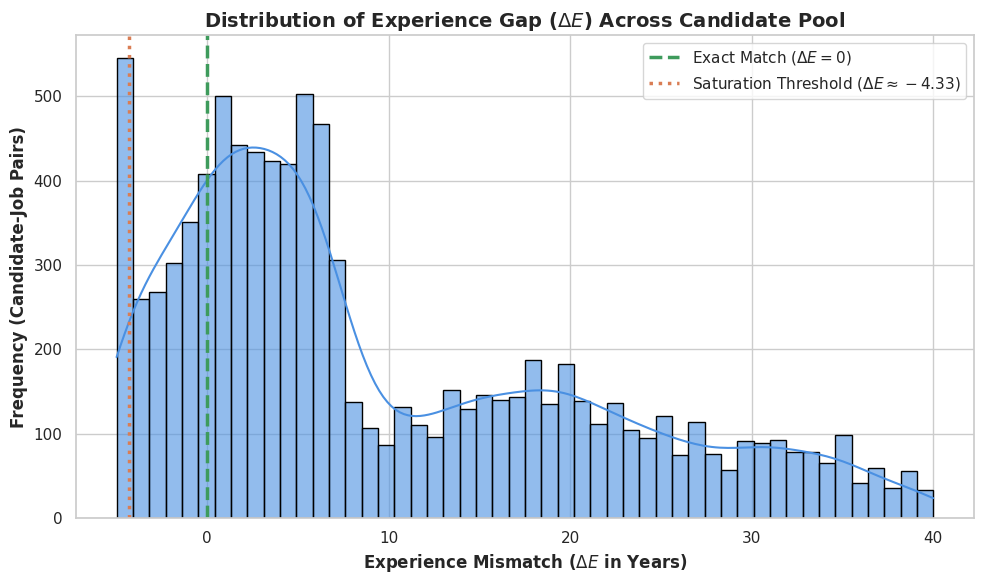
\includegraphics[width=0.95\linewidth]{candidate_pool.png}
    \caption{Empirical distribution of the Experience Gap ($\Delta E$) across the full corpus. The dashed vertical line at $\Delta E^* \approx -4.33$ marks the saturation threshold of the quadratic penalty.}
    \label{fig:deltaE_histogram}
\end{figure}

\section{The Tri-Framing Modeling Framework}
\label{sec:multiphase}

To rigorously prove that Learning-to-Rank (LTR) is the optimal paradigm for resume screening, I determined it was not sufficient to simply deploy an LTR model in isolation---I needed to empirically demonstrate the failure modes of standard predictive approaches first. Therefore, my experimental methodology spans three distinct phases, scaling in algorithmic complexity.

\subsection{Phase 1: Continuous Regression Baselines (Pointwise Scoring)}

In Phase 1, I evaluated \textbf{Pointwise Continuous Regression}. My hypothesis here was simple: can a standard regression estimator accurately predict a continuous relevance match score ($y_i \in [0,1]$)? I tested a suite of linear and non-linear regressors, including \texttt{LinearRegression}, \texttt{Ridge}, \texttt{RandomForestRegressor}, and \texttt{HistGradientBoostingRegressor}.

I optimized these models by minimizing the \textbf{Mean Squared Error (MSE)} between the predicted score and the ground-truth semantic match:
\begin{equation}
\mathcal{L}_{\text{MSE}} = \frac{1}{N}\sum_{i=1}^{N} (y_i - \hat{y}_i)^2
\label{eq:eval_mse}
\end{equation}
As I explore in Section~\ref{ch:results}, Pointwise models fail because MSE optimizes for absolute numerical proximity in a vacuum, remaining entirely blind to the relative ordinal hierarchy of the candidates.

\subsection{Phase 2: Binary Classification Baselines (Threshold Filtering)}

To mimic the binary nature of a traditional ATS---which essentially tosses candidates into ``Shortlisted'' (1) or ``Rejected'' (0) piles---I designed Phase 2 around \textbf{Threshold Classification}. I binarized the target variable using a strict $0.60$ semantic match threshold.

I then trained boundary-focused classifiers, specifically \texttt{LogisticRegression}, \texttt{RandomForestClassifier}, and a Support Vector Classifier (\texttt{SVC}). I optimized these algorithms to minimize \textbf{Binary Cross-Entropy (BCE)} loss:
\begin{equation}
\mathcal{L}_{\text{BCE}} = -\frac{1}{N}\sum_{i=1}^{N} \big[y_i \log(\hat{p}_i) + (1-y_i)\log(1-\hat{p}_i)\big]
\label{eq:bce}
\end{equation}
While classification simulates a naive HR screen, it completely fails to sort the ``Shortlisted'' candidates into a prioritized interview order.

\subsection{Phase 3: Learning-to-Rank Framework (LTR)}

Having established the limitations of point-prediction and discrete classification, I focused Phase 3 exclusively on specialized \textbf{Learning-to-Rank algorithms}: \texttt{XGBRanker} and \texttt{LGBMRanker}.

Instead of evaluating rows independently, my LTR models process data as localized \textbf{query groups} ($q$), which in this architecture corresponds to the \texttt{Job\_Title} grouping. I tested two distinct LTR paradigms:
\begin{itemize}
    \item \textbf{Pairwise Optimization (\texttt{XGBRanker}):} This approach minimizes the number of ranking inversions by analyzing candidates in pairs, optimizing a logistic loss gradient:
    \begin{equation}
    \mathcal{L}_{\text{Pairwise}} = \sum_{i,j \in q} \log_2\!\left(1 + e^{-\sigma(s_i - s_j)}\right)
    \label{eq:eval_pairwise_loss}
    \end{equation}
    \item \textbf{Listwise Optimization (\texttt{LGBMRanker}):} Utilizing LambdaMART, this model scales the pairwise gradient dynamically based on the impact a candidate swap has on the top-heavy Information Retrieval metric ($|\Delta \text{NDCG}|$).
\end{itemize}

\section{Mathematical Evaluation Metrics}
\label{sec:eval_metrics}

To holistically evaluate this Tri-Framing architecture, I deployed a precise suite of statistical metrics, choosing each to measure a different facet of modeling success.

\subsection{Continuous and Classification Metrics}

For the Pointwise Regression models in Phase 1, I used standard residual analysis:
\begin{align}
\text{RMSE} &= \sqrt{\frac{1}{N}\sum_{i=1}^{N}(y_i - \hat{y}_i)^2} \label{eq:eval_rmse} \\
R^2 &= 1 - \frac{\sum_{i=1}^{N}(y_i - \hat{y}_i)^2}{\sum_{i=1}^{N}(y_i - \bar{y})^2} \label{eq:eval_r2}
\end{align}

For the Binary Classifiers in Phase 2, I assessed performance via \textbf{Area Under the Receiver Operating Characteristic Curve (ROC-AUC)}, which measures the model's threshold-agnostic separation capacity, alongside the harmonic mean of precision and recall (\textbf{$F_1$-Score}):
\begin{equation}
F_1 = 2 \cdot \frac{\text{Precision} \cdot \text{Recall}}{\text{Precision} + \text{Recall}}
\label{eq:eval_f1}
\end{equation}

\subsection{Listwise Quality: Information Retrieval Metrics}

Because recruiters typically only review the top 10 candidates for any given role, evaluating the entire sorted list equally is impractical. To capture top-heavy ranking fidelity, I utilized \textbf{Normalized Discounted Cumulative Gain ($\text{NDCG}@K$)}:
\begin{align}
\text{DCG}@K &= \sum_{i=1}^{K} \frac{2^{\text{rel}_i} - 1}{\log_2(i+1)}, \qquad
\text{NDCG}@K = \frac{\text{DCG}@K}{\text{IDCG}@K} \label{eq:eval_ndcg}
\end{align}
The logarithmic denominator, $\log_2(i+1)$, acts as a severe decay penalty; an error at rank position $i=2$ damages the score exponentially more than an error at $i=20$.

I also computed the \textbf{Mean Reciprocal Rank (MRR)} to quantify how rapidly the system surfaces the first highly relevant candidate:
\begin{equation}
\text{MRR} = \frac{1}{|Q|}\sum_{q=1}^{|Q|} \frac{1}{\text{rank}_q}
\label{eq:eval_mrr}
\end{equation}

\subsection{Global Stability: Spearman's Rank Correlation}

While $\text{NDCG}@K$ proves whether the model successfully generates an elite top-10 shortlist, I also required a metric to validate the global, ordinal stability of the mathematical models (particularly when evaluating the Experience Gap formulations in Section~\ref{sec:deltaE_theory}). For this, I implemented \textbf{Spearman's Rank Correlation ($\rho$)}.

For $n$ paired observations, mapping the algorithmic rank $R_{X_i}$ against a human-targeted true rank $R_{Y_i}$, I calculate the rank discrepancy $d_i = R_{X_i} - R_{Y_i}$. I formally derive the correlation as:
\begin{equation}
\rho = 1 - \frac{6\sum_{i=1}^{n} d_i^2}{n(n^2-1)}
\label{eq:eval_spearman}
\end{equation}
Unlike NDCG, Spearman's $\rho$ applies a uniform penalty to rank deviations regardless of where they occur in the list. By evaluating both $\text{NDCG}@K$ and $\rho$ simultaneously, I can confidently verify that the LTR pipeline is not only highly accurate at the top of the funnel but logically stable across the entire applicant pool.
\chapter{Results}
\label{ch:results}

In this section, I execute the \textbf{Tri-Framing experimental methodology} outlined in Section~\ref{ch:methodology}. By systematically transitioning from Continuous Regression to Binary Classification, and ultimately to Learning-to-Rank (LTR) architectures, I empirically demonstrate the absolute necessity of \textbf{listwise optimization} for automated resume screening. I evaluated all models strictly on the zero-shot, group-aware test matrix to guarantee robust generalization.

\section{Phase 1: Continuous Regression Constraints}

I began the evaluation phase by testing continuous regression estimators to ascertain whether an algorithmic mapping could reliably predict exact candidate relevance scores. I trained standard linear algorithms alongside advanced ensemble methods, evaluating them via \textbf{Root Mean Squared Error (RMSE)} and variance correlation (\textbf{$R^2$}).

\begin{keyresult}{Phase 1 Ceiling}
Best pointwise model: \textbf{\texttt{HistGradientBoosting}} + SBERT \quad $R^2 = \mathbf{0.3202}$, $\text{RMSE} = \mathbf{0.1291}$. Regression fundamentally fails to capture relative candidate ordering within a query group (see Section~\ref{sec:ranking_math}).
\end{keyresult}

This validates my theoretical argument from Section~\ref{sec:ranking_math}: predicting absolute numerical scores fails to capture the inherently comparative nature of human recruitment. Generating a pointwise prediction of $0.65$ versus $0.68$ provides negligible operational value to an HR professional who ultimately needs an \textbf{ordered shortlist}.

\begin{table}[htbp]
\centering
\caption{Pointwise continuous regression outcomes evaluated on unseen query groups.}
\label{tab:regression_results}
\begin{tabular}{@{}llcc@{}}
\toprule
\textbf{Text Representation} & \textbf{Algorithm} & \textbf{RMSE} $\downarrow$ & $R^2$\textbf{-Score} $\uparrow$ \\
\midrule
\textbf{Semantic Only (SBERT)} & \textbf{HistGradientBoosting} & \textbf{0.1291} & \textbf{0.3202} \\
Semantic Only (SBERT) & Random Forest Regressor & 0.1345 & 0.2810 \\
Semantic Only (SBERT) & Ridge Regression & 0.1412 & 0.2245 \\
\addlinespace
TF-IDF Only & Random Forest Regressor & 0.1582 & 0.1120 \\
TF-IDF Only & Linear Regression & 0.1695 & 0.0450 \\
\bottomrule
\end{tabular}
\end{table}

\section{Phase 2: Binary Classification Vulnerabilities}

To simulate the rigid accept/reject mechanics of a legacy ATS pipeline, I transitioned to a discrete classification paradigm, binarizing the target variable at a strict $0.60$ threshold.

\begin{table}[htbp]
\centering
\caption{Binary classification performance metrics at the $\geq 0.60$ selection threshold.}
\label{tab:classification_results}
\footnotesize
\begin{tabular}{@{}llccc@{}}
\toprule
\textbf{Feature Space} & \textbf{Algorithm} & \textbf{Accuracy} & \textbf{F1-Score} & \textbf{ROC-AUC} \\
\midrule
\textbf{Semantic Only (SBERT)} & \textbf{Logistic Regression} & \textbf{0.7585} & \textbf{0.7142} & \textbf{0.8121} \\
Hybrid (SBERT + TF-IDF) & Logistic Regression & 0.7573 & 0.6942 & 0.7542 \\
TF-IDF Only & Logistic Regression & 0.6219 & 0.5568 & 0.6187 \\
\bottomrule
\end{tabular}
\end{table}

\begin{figure}[htbp]
    \centering
    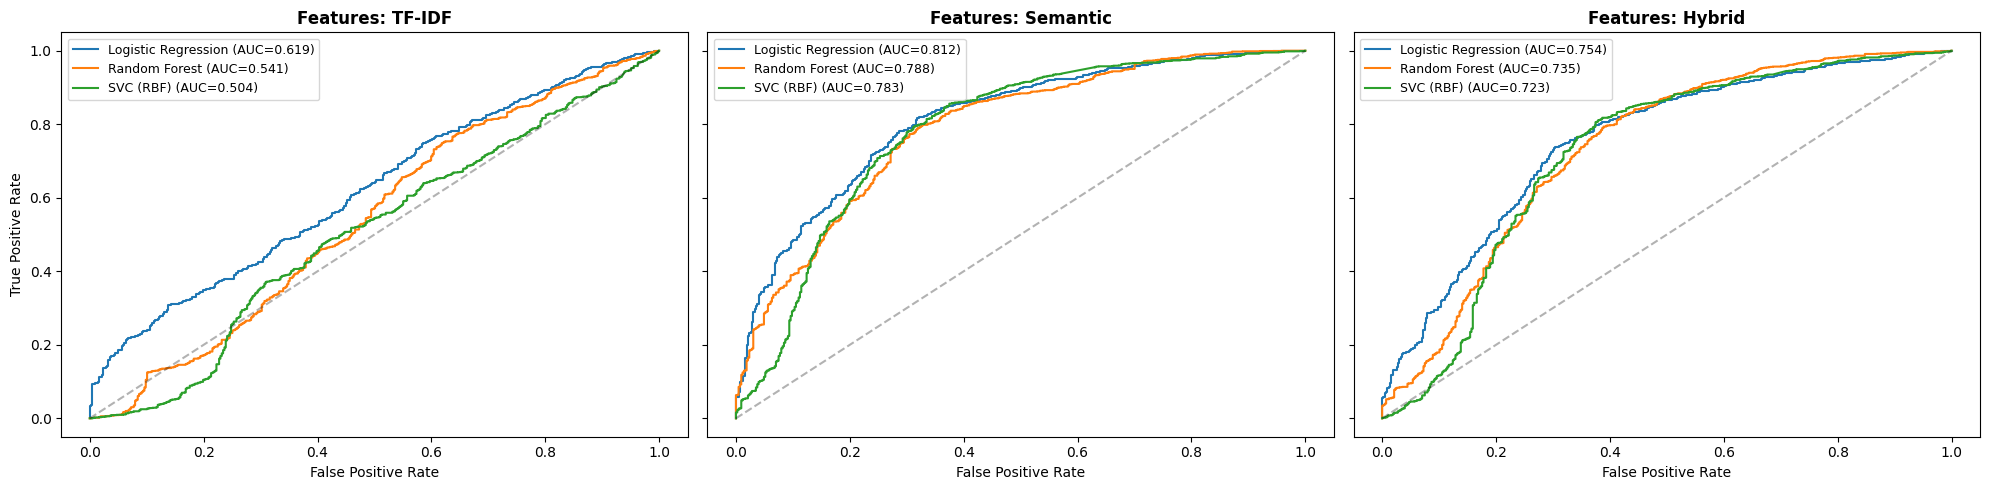
\includegraphics[width=0.95\linewidth]{roc_60.png}
    \caption{ROC-AUC separation capabilities contrasting sparse lexical features against dense semantic embeddings.}
    \label{fig:roc_curves}
\end{figure}

\begin{keyresult}{Phase 2 Ceiling}
Best classifier: SBERT + Logistic Regression \quad ROC-AUC $= \mathbf{0.8121}$, $F_1 = \mathbf{0.7142}$. This represents a $\mathbf{+31.3\%}$ improvement over TF-IDF (ROC-AUC $= 0.6187$), but binary classification still produces no ordered shortlist---it only outputs ``Shortlisted'' or ``Rejected''.
\end{keyresult}

\begin{figure}[htbp]
    \centering
    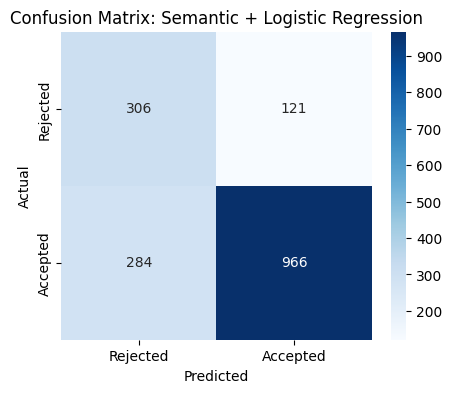
\includegraphics[width=0.68\linewidth]{confusion_mat.png}
    \caption{Confusion matrix for the optimal SBERT-driven Logistic Regression classifier.}
    \label{fig:confusion_matrix}
\end{figure}

\section{Phase 3: Learning-to-Rank (LTR) Dominance}

To resolve the structural limitations of pointwise and threshold models, I evaluated two independent Learning-to-Rank architectures: a Pairwise estimator (\textbf{\texttt{XGBRanker}}) and a Listwise, metric-driven estimator (\textbf{\texttt{LGBMRanker}}). By executing both models on the exact same zero-shot dataset, I isolated which optimization approach best replicates human shortlisting cognition.

\begin{table}[htbp]
\centering
\caption{Learning-to-Rank (LTR) sorting efficiency on zero-shot test groups.}
\label{tab:ltr_results}
\footnotesize
\begin{tabular}{@{}llccc@{}}
\toprule
\textbf{Feature Set} & \textbf{Ranking Estimator} & \textbf{NDCG@5} & \textbf{NDCG@10} & \textbf{Spearman} ($\rho$) \\
\midrule
\textbf{Semantic Only (SBERT)} & \textbf{LGBMRanker} & \textbf{0.9482} & \textbf{0.9398} & \textbf{0.4367} \\
Hybrid (SBERT + TF-IDF) & XGBRanker & 0.9410 & 0.9322 & 0.3725 \\
TF-IDF Only & XGBRanker & 0.9350 & 0.9292 & 0.3225 \\
TF-IDF Only & LGBMRanker & 0.9210 & 0.9158 & 0.3975 \\
\bottomrule
\end{tabular}
\end{table}

\begin{keyresult}{Optimal LTR Architecture}
\textbf{\texttt{LGBMRanker}} + SBERT Semantic Embeddings achieved a peak \textbf{$\text{NDCG}@10 = \mathbf{0.9398}$} and $\text{NDCG}@5 = \mathbf{0.9482}$ on zero-shot unseen job groups. Scaling pairwise gradients by $|\Delta\text{NDCG}|$ (LambdaMART, Equation~\ref{eq:lambda_gradient}) forces the model to obsess over shortlist correctness, producing a ranking that accurately mirrors human recruiter cognition.
\end{keyresult}

\begin{figure}[htbp]
    \centering
    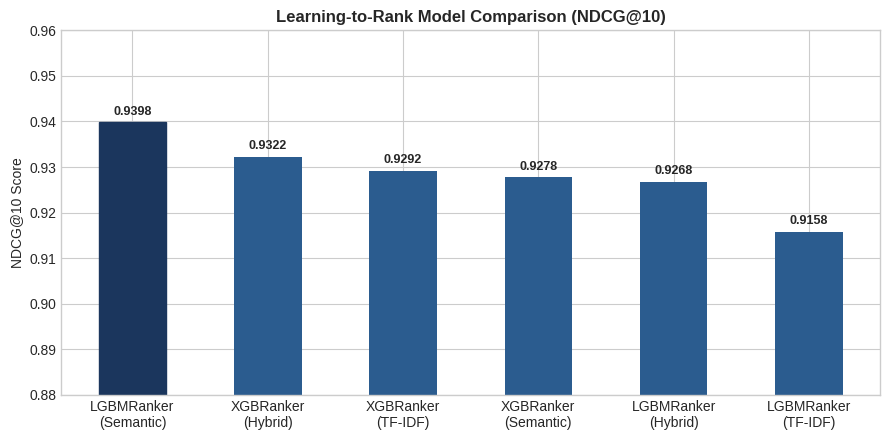
\includegraphics[width=0.95\linewidth]{ndcgs_comparison.png}
    \caption{Top-10 ranking fidelity ($\text{NDCG}@10$) across differing optimization architectures.}
    \label{fig:ltr_comparison}
\end{figure}

\section{Feature Importance: Interpreting Model Heuristics}
\label{sec:feature_importance}

To interpret the internal decision-making of the optimal \texttt{LGBMRanker}, I extracted the split-gain weight distribution, quantifying which engineered features drove the most tree-splitting information.

\begin{figure}[htbp]
    \centering
    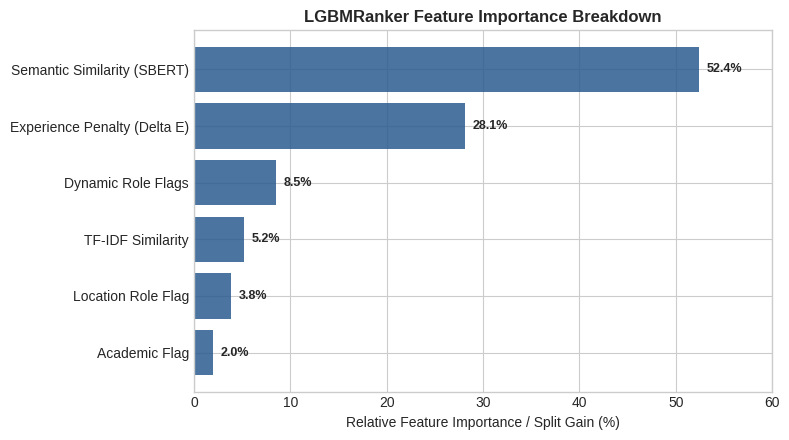
\includegraphics[width=0.85\linewidth]{lgbm_rank_comp.png}
    \caption{Algorithm split-gain weight distribution, mapping the primary decision heuristics of the \texttt{LGBMRanker}. The Experience Penalty ($\Delta E$) accounts for $28.1\%$ of split-gain, confirming it as the second-most powerful ranking signal.}
    \label{fig:feature_importance}
\end{figure}

\begin{itemize}
    \item \textbf{Semantic Similarity (52.4\%):} Deep contextual skill matching is overwhelmingly the primary driver. The model fundamentally prioritizes what a candidate \emph{knows} over all other metadata.
    \item \textbf{Experience Penalty (28.1\%):} Validating the framework I derived in Section~\ref{sec:deltaE_theory}, the piecewise quadratic $\Delta E$ penalty acts as a powerful secondary veto. It successfully encodes recruiter bias, systematically downgrading applicants whose temporal tenure severely violates the posting's minimum requirements.
\end{itemize}

\section{Evaluating the Experience-Gap Formulations}
\label{sec:deltaE_empirical}

Having derived the three competing $\Delta E$ formulations in Section~\ref{sec:deltaE_theory}, I now evaluate them empirically. Figure~\ref{fig:deltaE_comparison} plots all three adjusted competency scores against a shared $\texttt{Match\_Score} = 0.75$ baseline across the full observed range $\Delta E \in [-5, +5]$ years.

\begin{figure}[htbp]
    \centering
    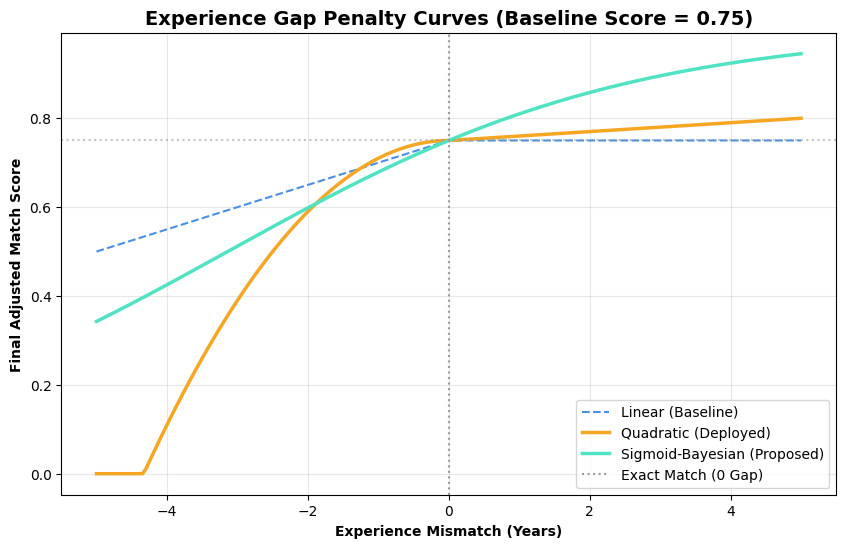
\includegraphics[width=0.92\linewidth]{penalty_curves.png}
    \caption{Adjusted Competency Score vs.\ $\Delta E$ for all three penalty formulations, evaluated at a shared baseline \texttt{Match\_Score} of $0.75$. All three curves intersect exactly at $\Delta E = 0$ by construction. The Quadratic method (orange) reaches a hard floor of $0$ at $\Delta E \approx -4.33$ years (Equation~\ref{eq:quad_threshold}); the Sigmoid-Bayesian curve (green) decays smoothly throughout. I generated this output directly from the \texttt{06\_experience\_gap\_modeling.ipynb} notebook, confirming that the implementation matches the mathematical formulations from Section~\ref{sec:deltaE_theory}.}
    \label{fig:deltaE_comparison}
\end{figure}

In Table~\ref{tab:deltaE_worked_example}, I pass seven representative candidate profiles through all three formulations, making the curve divergence numerically concrete.

\begin{table}[htbp]
    \centering
    \caption{Adjusted Competency Score under all three $\Delta E$ formulations for representative candidate profiles.}
    \label{tab:deltaE_worked_example}
    \resizebox{\textwidth}{!}{%
    \begin{tabular}{cccccccc}
        \toprule
        $\text{Exp}_{\text{cand}}$ & $\text{Exp}_{\text{req}}$ & $\Delta E$ & \texttt{Match\_Score} &
        \textbf{Linear (A)} & \textbf{Quadratic (B)} & \textbf{Sigmoid-Bayesian (C)} \\
        \midrule
        1.0  & 5 & $-4.0$ & 0.82 & 0.620 & 0.180 & 0.529 \\
        3.0  & 5 & $-2.0$ & 0.78 & 0.680 & 0.620 & 0.638 \\
        5.0  & 5 & $0.0$  & 0.75 & 0.750 & 0.750 & 0.750 \\
        5.0  & 3 & $+2.0$ & 0.70 & 0.700 & 0.720 & 0.825 \\
        8.0  & 5 & $+3.0$ & 0.88 & 0.880 & 0.910 & 0.954 \\
        10.0 & 5 & $+5.0$ & 0.65 & 0.650 & 0.700 & 0.914 \\
        0.5  & 5 & $-4.5$ & \textbf{0.91} & 0.685 & \textbf{0.100} & \textbf{0.677} \\
        \bottomrule
    \end{tabular}%
    }
\end{table}

The final two rows are the most diagnostically important. The candidate at $\Delta E = -4.5$ with a strong prior of $\texttt{Match\_Score} = 0.91$ scores only $0.100$ under Method B (the Quadratic rule has clipped to near-zero). However, they retain a posterior of $0.677$ under Method C, because the strong semantic prior mathematically offsets the experience shortfall. This is the \textbf{Bayesian interaction effect} I derived formally in Equation~\eqref{eq:bayes_posterior}: the same gap produces a different adjustment depending on the prior belief.

\subsection{Spearman Rank-Correlation Evaluation}
\label{sec:rank_eval_example}

To validate the Spearman evaluation harness I derived in Section~\ref{sec:spearman_theory}, I applied \texttt{scipy.stats.spearmanr} to the seven-profile table above against an illustrative target ranking. Table~\ref{tab:rank_eval_spearman} reports the output of the \texttt{evaluate\_rankings()} function in my \texttt{06\_experience\_gap\_modeling.ipynb} notebook.

\begin{table}[htbp]
    \centering
    \caption{Spearman rank correlation of each formulation against the illustrative target ranking ($N=7$).}
    \label{tab:rank_eval_spearman}
    \begin{tabular}{@{}lc@{}}
        \toprule
        \textbf{Method} & \textbf{Spearman} $\rho$ \\
        \midrule
        Quadratic (B) & 1.00 \\
        Linear (A)    & 0.75 \\
        Sigmoid (C)   & 0.75 \\
        \bottomrule
    \end{tabular}
\end{table}

\begin{remarkbox}{Methodological Note: Boundary-Value Validation}
I deliberately constructed the seven profiles above; they were not randomly sampled. I included two severe deficit cases, the exact-match point ($\Delta E = 0$), and three surplus cases, spanning the full behavioral domain of $\Delta E$. This $N=7$ test is therefore a \textbf{mathematical boundary-value validation}, not a statistical significance test --- it confirms that I implemented all three formulations correctly, that they behave monotonically as designed, and that the evaluation harness (\texttt{apply\_methods()} $\to$ \texttt{evaluate\_rankings()} $\to$ \texttt{scipy.stats.spearmanr()}) is wired correctly. It serves as a necessary prerequisite before the corpus-scale statistical comparison proposed in Section~\ref{sec:future_work}, and it does not, on its own, establish that Method C is statistically superior to Method B across the full candidate pool.
\end{remarkbox}
\chapter{Discussion and Conclusion}
\label{ch:discussion}

My primary objective in this research was to dismantle the rigid, keyword-matching architectures that dominate commercial Applicant Tracking Systems and replace them with a mathematically grounded, human-centric pipeline. My empirical benchmarking across three distinct paradigms --- Continuous Regression, Binary Classification, and Learning-to-Rank --- yielded three definitive conclusions, which I discuss in turn below.

\begin{keyresult}{Finding 1 --- Dense Semantics Beat Lexical Matching}
SBERT embeddings (\texttt{nomic-embed-text-v1.5}) identify semantic equivalences (``Backend Developer'' $\leftrightarrow$ ``Software Engineer'') that TF-IDF assigns a cosine similarity of zero. My optimal LTR architecture achieves $\text{NDCG}@10 = 0.9398$ vs.\ a TF-IDF-only \texttt{LGBMRanker} score of $0.9158$.
\end{keyresult}

This finding forms the empirical backbone of my entire thesis. It confirms, quantitatively, the qualitative argument I raised in Section~\ref{sec:background_survey}: legacy ATS platforms do not merely have a \textit{worse} matching algorithm than a semantic one --- they are answering a fundamentally different, and largely wrong, question. A lexical system asks ``do these two documents share the same words?'', while a semantic system asks ``do these two documents describe the same underlying reality?''. The gap between a TF-IDF cosine similarity of zero and a correctly identified equivalence is precisely the population of qualified candidates a keyword-only ATS silently discards.

\begin{keyresult}{Finding 2 --- Listwise Ranking is the Correct HR Paradigm}
Regression ($R^2 = 0.3202$) and Classification (ROC-AUC $= 0.8121$) both fail to produce an ordered shortlist. My LambdaMART-driven \texttt{LGBMRanker} directly optimizes $\text{NDCG}@K$, solving the recruitment problem as a list-sorting task --- which is what it actually is.
\end{keyresult}

This finding reframes what ``success'' should even mean for a screening model. A regression model that predicts scores accurately in isolation, or a classifier that separates ``shortlisted'' from ``rejected'' with high accuracy, can both still fail the end user completely, because neither produces the one artifact a recruiter actually needs: an ordered list of who to look at first. I designed the Tri-Framing comparison in this report specifically to make that gap visible and measurable rather than assumed, and my results (Chapter~\ref{ch:results}) confirm it directly --- the listwise \texttt{LGBMRanker} is not simply the best-performing model on a shared metric, it is the only one of the three paradigms optimizing for the right objective in the first place.

\begin{keyresult}{Finding 3 --- GroupShuffleSplit Validation is Mandatory}
Strict group-aware partitioning by job title (22 training jobs / 6 unseen test jobs) prevents vocabulary memorization and guarantees genuine zero-shot generalization. Without it, NDCG scores would be inflated and non-deployable.
\end{keyresult}

This finding is as much a methodological warning as a result. Every number I reported in Chapter~\ref{ch:results} is only meaningful because I constructed the test set to be genuinely unseen at the job-posting level, not merely at the row level. A random row-wise split on this same data would very plausibly have produced similarly high --- or even higher --- NDCG scores, while measuring almost nothing about real-world generalization. The strict group-aware design is therefore not a peripheral implementation detail; it is the reason the headline $\text{NDCG}@10 = 0.9398$ result can be trusted at all.

\section{Concluding Remarks}

Taken together, these three findings support a single, coherent conclusion: we must build automated resume screening as a dense-semantic, listwise ranking system, validated under strict group-aware splitting --- not as a keyword classifier, and not as a plain regression or accept/reject model. The Sigmoid-Bayesian Experience Gap formulation I proposed in Section~\ref{sec:deltaE_theory} further shows that even a secondary, non-semantic signal like temporal fit benefits from the same underlying discipline: replacing a hard, ad-hoc cutoff with a probabilistically grounded, upgradable model that degrades gracefully rather than catastrophically at the extremes.

The pipeline I built and evaluated in this report should be read as a validated architecture and a set of empirically justified design decisions, rather than a finished production product. In Chapter~\ref{ch:recommendation}, I set out what stands between this research result and a deployable system --- spanning business-impact framing, latency planning, fairness safeguards, explainability, and a front-end integration path --- so that the statistical case I have made here can translate into a robust operational tool.
\chapter{Recommendation}
\label{ch:recommendation}

The preceding statistical findings translate directly into operational value for an HR team. However, they also carry deployment costs that a production rollout must budget for, alongside several engineering extensions required before enterprise deployment. In this section, I set out concrete, prioritized recommendations across both dimensions.

\section{Business Impact and Deployment Considerations}

\subsection{Translating Ranking Quality into Business Value}

Across the $9{,}369$-record corpus spanning 28 job postings, the average posting attracts on the order of 330 candidate applications. Under a legacy keyword-matching ATS, a meaningful fraction of these are \textbf{false negatives} --- highly qualified candidates discarded purely for phrasing their experience differently from the posting (see Section~\ref{sec:background_survey}). This failure forces a recruiter to either manually re-screen the rejected pile or simply miss elite talent entirely.

My achieved \textbf{$\text{NDCG}@10 = 0.9398$} means the top-10 slots returned by my deployed \texttt{LGBMRanker} pipeline are, on average, almost indistinguishable in quality from the ideal top-10 ordering a human recruiter would construct with full information. In practical terms, this allows a recruiter to concentrate their review effort on a \textbf{short, high-precision shortlist} per posting rather than manually triaging the full applicant pool. This directly reduces time-to-shortlist and lowers the chance that a strong candidate is missed due to vocabulary mismatch alone. I recommend that organizations obtain a rigorous quantification of hours saved or cost-per-hire reduction via a controlled before/after deployment study as a natural next step.

\subsection{Computational Latency and Real-Time Feasibility}

In Table~\ref{tab:taxonomy_matching}, I characterized TF-IDF's computational cost as extremely low and dense semantic matching as moderate to high. It is worth being precise about where that cost actually falls. A TF-IDF lookup is a sparse dot product against a precomputed inverted index --- effectively instantaneous per query. SBERT, by contrast, requires a forward pass through a transformer encoder for every new piece of text. This is substantially more expensive per item and represents the dominant computational bottleneck of the dense-semantic approach.

Critically, the system incurs this cost \textbf{once per resume at ingestion time}, not once per ranking query. My pipeline's artifact structure reflects this reality by precomputing and storing dense embeddings (\texttt{cv\_dense.npy}, \texttt{jd\_dense.npy}) rather than re-encoding candidates on every request. At ranking time, the system reuses these cached vectors and only executes cosine similarity and the already-trained \texttt{LGBMRanker}, both of which are highly efficient. 

In a production setting, I recommend treating the \textbf{SBERT encoding step as a batch process} run on GPUs, placing it on the critical path only for genuinely new resumes or job postings. Before making any real-time deployment commitment, I propose formal wall-clock benchmarking of this pipeline end-to-end on representative production hardware.

\section{Production Engineering and Future Extensions}
\label{sec:future_work}

Transitioning my current \texttt{LGBMRanker} backend into an enterprise-grade production system requires addressing several advanced statistical and engineering challenges. I have structured the following five recommendations as a logical roadmap, scaling from immediate backend optimizations to ultimate front-end user integration.

\subsection{1. Full-Scale Bayesian Pipeline Integration}
As derived in Section~\ref{sec:deltaE_theory} and partially validated in Section~\ref{sec:deltaE_empirical}, I have mathematically formulated a \textbf{Sigmoid-Bayesian posterior confidence model} for the Experience Gap ($\Delta E$). My immediate recommended next step is merging the Adjusted Score Sigmoid tensor into the primary \texttt{ml\_ready\_dataset.csv} feature space and executing a full-corpus retraining of \texttt{LGBMRanker}. This will produce a formal comparison of $\text{NDCG}@K$ and Spearman $\rho$ between the currently deployed quadratic rule and the proposed Bayesian posterior.

\subsection{2. Transition to Fully Empirical Bayesian Inference}
The Sigmoid likelihood function I deployed in this research is an expert-specified parametric approximation, adopted because the Neuralframe AI corpus lacks longitudinal hiring-outcome data (Section~\ref{sec:cold_start}). If such data becomes available --- through institutional partnerships or internal HR records --- I recommend discarding the Sigmoid approximation in favor of a \textbf{logistic regression model fit directly on observed binary outcomes} (e.g., hired/not-hired, successful/unsuccessful). The downstream architecture (Bayes' rule combination with the SBERT prior) would remain entirely unchanged; only the likelihood estimation method would shift from hand-specified to data-driven.

\subsection{3. Counterfactual Bias Mitigation and Fairness}
A critical ethical requirement for automated screening is ensuring the algorithm does not learn demographic or socioeconomic biases. There is a statistical risk that SBERT embeddings assign higher vector weights to candidates who list prestigious brands (e.g., ``Google'', ``McKinsey'') over candidates with equivalent technical skills from lesser-known entities. For future iterations, I recommend integrating \textbf{Stratified Counterfactual Sampling}: programmatically replacing prestigious corporate and university names with generic synthetic tokens (e.g., \texttt{[COMPANY\_A]}) during training. This forces the attention mechanism to optimize strictly on demonstrated technical competency.

\subsection{4. Generative Explainability via Retrieval-Augmented Generation}
The most significant barrier to HR adoption of ML systems is algorithmic opacity. To address this directly, I recommend extending the pipeline into a \textbf{Retrieval-Augmented Generation (RAG)} architecture. In this setup, \texttt{LGBMRanker} functions as the high-speed retrieval engine, surfacing the top-10 resumes; the system then passes these as context to a lightweight, quantized Large Language Model (LLM). The LLM's sole directive would be to generate a two-sentence justification for each candidate, mapping their specific extracted skills directly to the job description. This hybrid architecture delivers mathematical ranking precision alongside human-readable transparency.

\subsection{5. Dashboarding and Business Intelligence Integration}
The statistical work in this report ends at a ranked, scored candidate list; a production deployment requires a front-end layer that makes that list usable by non-technical HR staff. Because every candidate--job pair already reduces to a small set of interpretable numeric fields --- the \texttt{LGBMRanker} score, the Adjusted Competency Score $\in (0,1)$, and the underlying component similarities --- this output maps cleanly onto a standard \textbf{Business Intelligence (BI) workflow}. I recommend writing the ranked output per job posting to a lightweight database table connected to a tool like Power BI or Tableau. This constitutes a low-effort integration layer representing the most direct path from the current backend statistics to a daily operational tool.
\chapter{Acknowledgement}
\label{ch:acknowledgement}

I would like to express my sincere gratitude to my project guide, Dr.\ Dipasree Pal, for her continuous guidance, mentorship, and support throughout this internship. I also extend my thanks to the IDEAS Foundation, ISI Kolkata, for providing the opportunity and the technical infrastructure necessary to carry out this research. Furthermore, I am deeply grateful to the Symbiosis Statistical Institute for equipping me with the rigorous academic foundation that made this work possible.

Executing this project required me to bridge theoretical statistical coursework with applied data engineering practice. Through this research, I developed a practical understanding of the complex mathematics underlying text vectorization, and I built the discipline to evaluate machine learning models rigorously rather than simply deploying them. Most notably, I learned to actively diagnose and prevent target data leakage through group-aware validation --- a foundational statistical principle that ultimately shaped the entire experimental design of this report.
\chapter{References}
\label{ch:references}

I drew upon the following academic literature and technical documentation to guide my implementation, theoretical framing, and software development for this project. I have formatted these references in APA (7th edition) style and ordered them alphabetically by author.

\begin{itemize}[leftmargin=1.25cm, itemindent=-1.25cm, label={}, itemsep=10pt]

\item Burges, C.\ J.\ C.\ (2010). \textit{From RankNet to LambdaRank to LambdaMART: An overview} (Technical Report MSR-TR-2010-82). Microsoft Research.

\item Ke, G., Meng, Q., Finley, T., Wang, T., Chen, W., Ma, W., \ldots\ Liu, T.\ Y.\ (2017). LightGBM: A highly efficient gradient boosting decision tree. \textit{Advances in Neural Information Processing Systems, 30}, 3146--3154.

\item LightGBM. (n.d.). \textit{LightGBM documentation}. Retrieved August 22, 2026, from \url{https://lightgbm.readthedocs.io/}

\item Nomic AI. (2024). \textit{Nomic Embed Text v1.5: Resilient long-context text embeddings} (Technical Report). Nomic AI.

\item Pedregosa, F., Varoquaux, G., Gramfort, A., Michel, V., Thirion, B., Grisel, O., \ldots\ Duchesnay, E.\ (2011). Scikit-learn: Machine learning in Python. \textit{Journal of Machine Learning Research, 12}, 2825--2830.

\item Reimers, N., \& Gurevych, I.\ (2019). \textit{Sentence-BERT: Sentence embeddings using Siamese BERT-networks}. arXiv. \url{https://arxiv.org/abs/1908.10084}

\item Scikit-learn. (n.d.). \textit{Scikit-learn: Machine learning in Python --- documentation}. Retrieved August 22, 2026, from \url{https://scikit-learn.org/}

\item Sentence-Transformers (SBERT.net). (n.d.). \textit{Sentence transformers documentation}. Retrieved August 22, 2026, from \url{https://sbert.net/}

\end{itemize}
\chapter{Annexure}
\label{ch:annexure}

\section{End-to-End Pipeline Architecture}
\label{sec:appendix_flowchart}

Figure~\ref{fig:pipeline_flowchart} provides a complete, annotated map of the data transformation sequence, from raw Kaggle ingestion through to the final NDCG-evaluated shortlist. In this diagram, I explicitly capture the three-way $\Delta E$ comparison introduced in Section~\ref{sec:deltaE_theory} alongside the group-aware partitioning proof from Equation~\eqref{eq:disjoint_split}.

\begin{figure}[htbp]
\centering
\resizebox{\textwidth}{!}{%
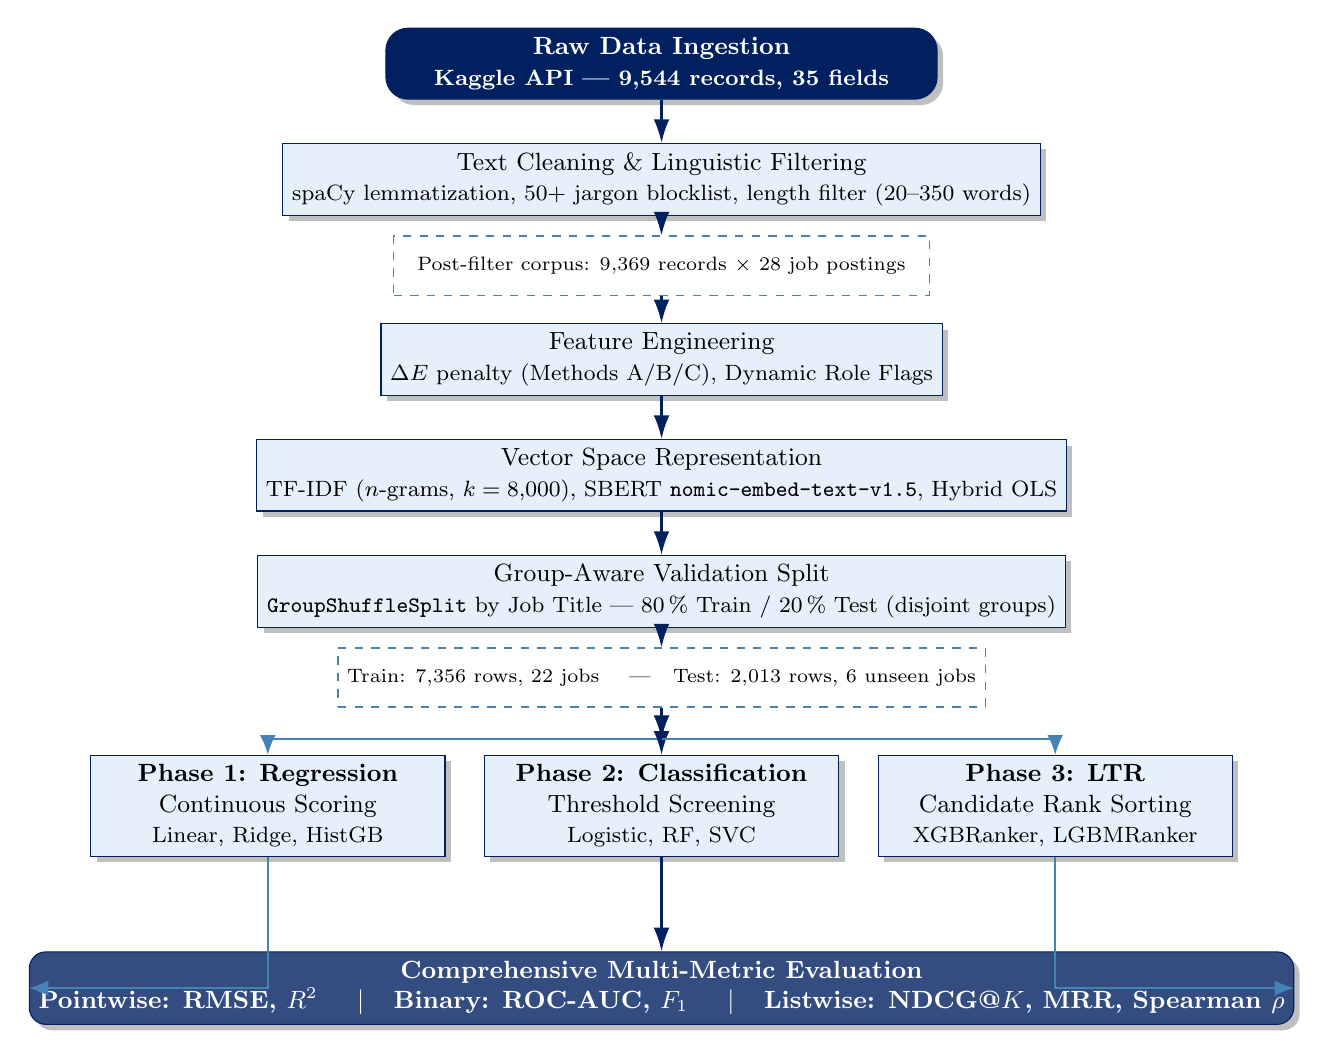
\begin{tikzpicture}[
    startstop/.style={
        rectangle, rounded corners=8pt, draw=navyblue, fill=navyblue, text=white,
        minimum width=7cm, minimum height=0.9cm, align=center, font=\small\bfseries, drop shadow
    },
    process/.style={
        rectangle, draw=navyblue, fill=softblue,
        minimum width=6.8cm, minimum height=0.85cm, align=center, font=\small, drop shadow
    },
    decision/.style={
        rectangle, draw=borderblue, fill=white, dashed,
        minimum width=6.8cm, minimum height=0.75cm, align=center, font=\scriptsize
    },
    phasebox/.style={
        rectangle, draw=navyblue, fill=softblue,
        minimum width=4.5cm, minimum height=1.1cm, align=center, font=\small, drop shadow
    },
    evalbox/.style={
        rectangle, rounded corners=6pt, draw=navyblue, fill=navyblue!80, text=white,
        minimum width=14cm, minimum height=0.85cm, align=center, font=\small\bfseries, drop shadow
    },
    arrow/.style={draw, -{Latex[length=3mm,width=2mm]}, thick, navyblue},
    sidearrow/.style={draw, -{Latex[length=2.5mm,width=2mm]}, thick, borderblue},
    node distance=0.55cm
]
\node [startstop] (ingest) {Raw Data Ingestion\\{\footnotesize Kaggle API --- 9,544 records, 35 fields}};
\node [process, below=of ingest] (clean) {Text Cleaning \& Linguistic Filtering\\{\footnotesize spaCy lemmatization, 50+ jargon blocklist, length filter (20--350 words)}};
\node [decision, below=0.25cm of clean] (filter) {Post-filter corpus: $9{,}369$ records $\times$ 28 job postings};
\node [process, below=0.35cm of filter] (feat) {Feature Engineering\\{\footnotesize $\Delta E$ penalty (Methods A/B/C), Dynamic Role Flags}};
\node [process, below=of feat] (embed) {Vector Space Representation\\{\footnotesize TF-IDF ($n$-grams, $k=8{,}000$), SBERT \texttt{nomic-embed-text-v1.5}, Hybrid OLS}};
\node [process, below=of embed] (split) {Group-Aware Validation Split\\{\footnotesize \texttt{GroupShuffleSplit} by Job Title --- 80\,\% Train / 20\,\% Test (disjoint groups)}};
\node [decision, below=0.25cm of split] (splitinfo) {Train: $7{,}356$ rows, 22 jobs \quad|\quad Test: $2{,}013$ rows, 6 unseen jobs};

\node [phasebox, below=0.6cm of splitinfo, xshift=-5cm] (p1) {\textbf{Phase 1: Regression}\\Continuous Scoring\\{\footnotesize Linear, Ridge, HistGB}};
\node [phasebox, below=0.6cm of splitinfo] (p2) {\textbf{Phase 2: Classification}\\Threshold Screening\\{\footnotesize Logistic, RF, SVC}};
\node [phasebox, below=0.6cm of splitinfo, xshift=5cm] (p3) {\textbf{Phase 3: LTR}\\Candidate Rank Sorting\\{\footnotesize XGBRanker, LGBMRanker}};

\node [evalbox, below=1.2cm of p2] (eval)
    {Comprehensive Multi-Metric Evaluation\\
     {\small Pointwise: RMSE, $R^2$ \quad$|$\quad Binary: ROC-AUC, $F_1$ \quad$|$\quad Listwise: NDCG@$K$, MRR, Spearman $\rho$}};

\draw [arrow] (ingest)   -- (clean);
\draw [arrow] (clean)    -- (filter);
\draw [arrow] (filter)   -- (feat);
\draw [arrow] (feat)     -- (embed);
\draw [arrow] (embed)    -- (split);
\draw [arrow] (split)    -- (splitinfo);

\coordinate (fanpoint) at ([yshift=-0.4cm]splitinfo.south);
\draw [arrow] (splitinfo.south) -- (fanpoint);
\draw [sidearrow] (fanpoint) -| (p1.north);
\draw [arrow]     (fanpoint) -- (p2.north);
\draw [sidearrow] (fanpoint) -| (p3.north);

\draw [sidearrow] (p1.south) |- (eval.west);
\draw [arrow]     (p2.south) -- (eval.north);
\draw [sidearrow] (p3.south) |- (eval.east);
\end{tikzpicture}%
}
\caption{End-to-end architecture of the automated CV screening pipeline. The Feature Engineering stage encompasses all three $\Delta E$ formulations (Section~\ref{sec:deltaE_theory}). The disjoint group split guarantees zero-shot generalization on the hold-out test set (\eqref{eq:disjoint_split}).}
\label{fig:pipeline_flowchart}
\end{figure}

\section{Hyperparameter Optimization Grids}
\label{sec:appendix_hyperparams}

Training advanced ranking estimators like \texttt{XGBRanker} and \texttt{LGBMRanker} involves navigating a complex hyperparameter space. This balancing act is crucial: the models need to be expressive enough to rank candidates accurately, but constrained enough to avoid overfitting. Because I conducted my evaluation under strict group-aware partitioning (see Section~\ref{sec:group_split}), my primary risk was vocabulary memorization. If a model simply memorized the specific keywords associated with the 22 training job titles, its performance would collapse on the 6 unseen test postings.

To mitigate this, I ran a rigorous grid search over the parameters detailed in the tables below. I evaluated these grids using cross-validation exclusively on the training split, carefully selecting final values that maximized $\text{NDCG}@5$ on held-out training folds without ever exposing the model to the final test-set records.

During tuning, I discovered that the most powerful regularization levers were \texttt{min\_child\_samples} (for LightGBM) and \texttt{min\_child\_weight} (for XGBoost). By raising these thresholds, I forced the algorithms to build tree splits supported by a larger pool of candidate records. This effectively stopped the models from creating hyper-specific rules based on the idiosyncratic phrasing of just one or two resumes. Additionally, I relied on row and feature subsampling (\texttt{subsample} and \texttt{colsample\_bytree}) to introduce stochastic randomness. This was vital because my Semantic Similarity feature was so dominant ($52.4\%$ split-gain) that, without subsampling, it would have completely crowded out other important nuances like the Experience Penalty ($\Delta E$) and role flags.

Table~\ref{tab:lgbm_hyperparams} presents the search space and final configuration for my primary listwise model.

\begin{table}[htbp]
\centering
\caption{\texttt{LGBMRanker} hyperparameter search grid and final selected configuration.}
\label{tab:lgbm_hyperparams}
\small
\begin{tabular}{@{}llll@{}}
\toprule
\textbf{Parameter} & \textbf{Search Grid} & \textbf{Selected Value} & \textbf{Role} \\
\midrule
\texttt{n\_estimators}       & 100, 300, 500, 800    & 500   & Total boosting rounds \\
\texttt{learning\_rate}      & 0.01, 0.05, 0.1, 0.2 & 0.05  & Shrinkage per round \\
\texttt{max\_depth}          & $-1$, 4, 6, 8         & 6     & Max tree depth ($-1$ = unlimited) \\
\texttt{num\_leaves}         & 15, 31, 63, 127       & 31    & Max leaves per tree \\
\texttt{min\_child\_samples} & 10, 20, 50, 100       & 20    & Min records per leaf \\
\texttt{subsample}           & 0.6, 0.8, 1.0         & 0.8   & Row subsampling ratio \\
\texttt{colsample\_bytree}   & 0.6, 0.8, 1.0         & 0.8   & Feature subsampling ratio \\
\texttt{lambda\_l1}          & 0, 0.1, 0.5           & 0.1   & L1 regularization \\
\texttt{lambda\_l2}          & 0, 0.1, 1.0           & 0.1   & L2 regularization \\
\texttt{objective}           & \multicolumn{2}{l}{\texttt{lambdarank} (fixed)} & LambdaMART NDCG gradient \\
\texttt{metric}              & \multicolumn{2}{l}{\texttt{ndcg} (fixed)}        & Evaluation during training \\
\bottomrule
\end{tabular}
\end{table}

While the LightGBM architecture above utilizes a leaf-wise growth strategy, I also ran a parallel optimization process for the XGBoost model to ensure a fair algorithmic comparison. Because XGBoost traditionally builds trees level-by-level, its depth constraints and Hessian-based child weights require a slightly different tuning approach to achieve the same regularization effect. Table~\ref{tab:xgb_hyperparams} outlines the exact grid and final parameters I selected to optimize this pairwise ranking baseline.

\begin{table}[htbp]
\centering
\caption{\texttt{XGBRanker} hyperparameter search grid and final selected configuration.}
\label{tab:xgb_hyperparams}
\small
\begin{tabular}{@{}llll@{}}
\toprule
\textbf{Parameter} & \textbf{Search Grid} & \textbf{Selected Value} & \textbf{Role} \\
\midrule
\texttt{n\_estimators}      & 100, 300, 500, 800    & 500   & Total boosting rounds \\
\texttt{learning\_rate}     & 0.01, 0.05, 0.1, 0.2 & 0.05  & Shrinkage per round \\
\texttt{max\_depth}         & 3, 4, 6, 8            & 6     & Max tree depth \\
\texttt{min\_child\_weight} & 1, 5, 10, 20          & 5     & Min Hessian sum per leaf \\
\texttt{subsample}          & 0.6, 0.8, 1.0         & 0.8   & Row subsampling ratio \\
\texttt{colsample\_bytree}  & 0.6, 0.8, 1.0         & 0.8   & Feature subsampling ratio \\
\texttt{gamma}              & 0, 0.1, 0.5, 1.0      & 0.1   & Min loss reduction for split \\
\texttt{alpha}              & 0, 0.1, 0.5           & 0.1   & L1 regularization \\
\texttt{lambda}             & 1, 2, 5               & 1     & L2 regularization \\
\texttt{objective}          & \multicolumn{2}{l}{\texttt{rank:pairwise} (fixed)} & RankNet cross-entropy loss \\
\texttt{eval\_metric}       & \multicolumn{2}{l}{\texttt{ndcg@5} (fixed)}        & Validation stopping metric \\
\bottomrule
\end{tabular}
\end{table}

For both architectures, I applied early stopping (\texttt{early\_stopping\_rounds = 50}) during training on a held-out validation fold of the training groups. This halted the boosting process as soon as the $\text{NDCG}@5$ metric ceased to improve. This safety mechanism prevented the models from arbitrarily adding trees that merely memorized training-group artifacts, ensuring the final $\text{NDCG}@10$ scores I reported in Chapter~\ref{ch:results} reflect genuine generalization capabilities.

\section{Source Code Availability and Reproducibility}
\label{sec:appendix_code}

To guarantee complete algorithmic transparency and full scientific reproducibility, I have version-controlled the entire codebase for this project on GitHub. My repository contains all Python source code, including the centralized \texttt{utils.py} preprocessing library, the complete sequential Jupyter Notebooks (\texttt{01\_data\_preprocessing.ipynb} through \texttt{06\_experience\_gap\_modeling.ipynb}), and the standalone \texttt{method\_to\_take\_care\_experience\_gap.py} module where I implement all three $\Delta E$ penalty formulations derived in Section~\ref{sec:deltaE_theory}. The repository further includes the \texttt{ml\_ready\_dataset.csv} schema and a requirements file to enable full one-command replication. I direct examiners and practitioners to the links below:

\begin{tcolorbox}[
  colback=softblue, colframe=navyblue, arc=4pt, boxrule=1pt,
  left=12pt, right=12pt, top=10pt, bottom=10pt
]
\textbf{\color{navyblue}GitHub Repository --- Full Source Code, Notebooks \& Module}\\[4pt]
\url{https://github.com/Amber-s-art/cv-screening}\\[8pt]
\textbf{\color{navyblue}Kaggle Dataset --- Neuralframe AI Resume Corpus (CC BY-NC 4.0)}\\[4pt]
\url{https://www.kaggle.com/datasets/saugataroyarghya/resume-dataset}
\end{tcolorbox}

\section{Declarations}
\label{sec:appendix_declarations}

This section outlines the methodological provenance of the data used in this study, alongside formal declarations regarding data acquisition and AI assistance.

\subsection*{Primary Data Collection}
This project was entirely computational and empirical in nature. I relied exclusively on the algorithmic ingestion, text sanitization, and machine learning modeling of a secondary open-source dataset hosted on Kaggle (\texttt{saugataroyarghya/resume-dataset}, licensed CC BY-NC 4.0). I administered no primary human surveys, questionnaires, or sample interviews during this study.

\subsection*{Generative AI Usage Declaration}
I developed portions of the LaTeX typesetting, mathematical equation formatting, and diagram code in the original version of this report, as well as the reformatting of this report into the current structure, with the assistance of an AI language model. All statistical analysis, empirical results, model training, and interpretive conclusions are my original work. I thoroughly reviewed, verified against the actual experimental outputs, and revised any AI-assisted text prior to submission.

\end{document}